\documentclass[a4paper, 13pt]{scrreprt}
\usepackage[utf8]{inputenc} 
\usepackage{amssymb}
\usepackage[ngerman]{babel}
\usepackage{amsthm}
\usepackage{amsmath}
\usepackage{graphicx}
%\usepackage{pstricks}
\usepackage[T1]{fontenc}
\usepackage{color}
\usepackage{lmodern}
\usepackage[pdfborder={0 0 0}]{hyperref}

\pagestyle{headings}

\newtheorem{satz}{Satz}[section]
\newtheorem{theorem}{Theorem}[section]
\newtheorem{lemma}[theorem]{Lemma}
\newtheorem{proposition}[theorem]{Proposition}
\newtheorem{corollar}[theorem]{Corollar}
\theoremstyle{definition} \newtheorem{definition}{Definition}[section]

\newenvironment{beweis}[1][Beweis]{\begin{trivlist}
\item[\hskip \labelsep {\bfseries #1}]}{\end{trivlist}}
\newenvironment{beispiel}[1][Beispiel]{\begin{trivlist}
\item[\hskip \labelsep {\bfseries #1}]}{\end{trivlist}}
\newenvironment{bemerkung}[1][Bemerkung]{\begin{trivlist}
\item[\hskip \labelsep {\bfseries #1}]}{\end{trivlist}}

\DeclareMathOperator*{\argmin}{arg\,min}

\newcommand{\RR}{\mathbb{R}}

\begin{document}
\title{Nichtlineare Dynamik}
\publishers{\small{Fehler in der Mitschrift an
\url{alexander.book@gmx.de}} oder 
\url{dominik.o@gmx.net}}
\maketitle
\tableofcontents


\chapter{Grundlagen}
\section{Dynamische Systeme}
\begin{definition}[dynamische Systeme]
Wir behandeln zwei Arten von dynamischen Systemen:
\begin{enumerate}
\item \emph{kontinuierliches dynamisches System}: Es gibt eine kontinulierliche Zeitvariable $t\in\mathbb{R}$
\item \emph{diskretes dynamisches System}: Es gibt eine kontinulierliche Zeitvariable $t\in\mathbb{Z}$
\end{enumerate}
Im folgenden bezeichnet $T$ entweder $\mathbb{R}$ oder $\mathbb{Z}$, je nachdem, welches dynamische System im Kontext verwendet wird.

Es gibt einen \emph{(Zustands-)Phasenraum} $X$, der den Zustand eines Systems mit verschiedenen Gr"o"sen beschreibt $(X\subseteq \mathbb{R}^n, n\in \mathbb{N})$. $x\in X$ beschreibt somit einen m"oglichen Zustand eines \emph{dynamischen Systems}. Falls $\operatorname{dim}(X) < \infty$, so nennt man es \emph{endlich dimensionales dynamisches System}. Andernfalls ($\operatorname{dim}(X) = \infty$) nennt man es \emph{unendlich dimensionales dynamisches System}. Mit \emph{Dynamik} bezeichnet man die zeitliche Ver"anderung des Zustands eines dynamischen Systems.
\end{definition}


Generell beginnt ein dynamisches System bei einer Anfangszeit $t_o$ und einem Zustand $x(t_0) = x_0 \in X$. Anhand dieses Punktes wird jedem andern Zeitpunkt ein eindeutiger Zustand zugewiesen ($x(t_0) = x_0 \Rightarrow \forall t\in T\  \exists! x_t\in\mathbb{R}^n: x(t) = x_t$)
Diese Zuordnung wird durch die \emph{Flussabbildung} definiert:
$$\phi\colon \mathbb{R}\times X\to X, \ \forall t \in T: x(t):= \phi(t-t_0, x_0) $$


\begin{definition}[Klassifikation von dynamischen Systemen]
Man unterscheidet dynamische Systeme in lineare und nicht-lineare Systeme:
\begin{enumerate}
\item \emph{Lineares dynamisches System}: $\phi(t, \cdot)\colon X \to X$ ist linear. Man schreibt dann auch $\phi(t, x) = \phi(t)x$. Dabei ist $\phi(t)$ ein linearer Operator f"ur alle $t\in T$
\item \emph{Nichtlineares dynamisches System}: $\phi(t, \cdot)\colon X \to X$ ist nicht linear.
\end{enumerate}
\end{definition}
\begin{definition}[Phasendiagramm]
Durch ein dynamischen Systems $(X,\phi)$ wird jedem Zustand $x\in X$ ein \emph{Orbit} zugeordnet:
$$\Gamma_x := \left \{\left. y \in X \right | \exists t\in T: \phi(t,x) = y\right \}$$ 
Ein \emph{Phasendiagramm} ist die Skizze des Orbits $\Gamma_x$ f"ur einige $x \in X$.
\begin{description}
\item[Bemerkung]Durch jeden Punkt $x\in X$ verl"auft genau ein Orbit $\Gamma_x$. Insbesondere k"onnen sich Orbits nicht traversal (selbst) schneiden.
\end{description}
\end{definition}
\subsection{Eigenschaften der Flussabbildung $\phi$}
Die Flussabbildung gen"ugt folgenden Eigenschaften:
\begin{enumerate}
\item $\forall x\in X: \phi(0,x) = x$
\item $\phi(\cdot, x)$ ist stetig f"ur alle $x\in X$.
\item $\phi(t, \cdot)$ ist stetig f"ur alle $t\in T$.
\item $\phi(t, \cdot)\colon X \to X$ ist ein Hom"oomorphismus (d.h. bijektiv und Umkehrabbildung ist stetig)
\item $\phi(s+t, x) = \phi\left(s, \phi(t,x)\right)$ f"ur alle $s,t \in T,\  x\in X$
\end{enumerate}

\section{Elementarste Typen von dynamischen Systemen}
Dynamische Systeme k"onnen auch implizit angegeben werden. Im Folgenden werden die zwei wichtigsten dynamischen Systeme f"ur diese Vorlesung vorgestellt.
\subsection{Gew"ohnliche Differentialgleichungs Systeme (GDG-Systeme)}
GDG-Systeme sind ein Beispiel f"ur kontinuierliche dynamische Systeme. Betrachtet man eine autonome gew"ohnliche Differentialgleichung 1. Ordnung
$$\dot x= v(x)$$
wobei $v\colon\mathbb{R}^n\to\mathbb{R}^n$ ein Vektorfeld ist. Durch das zugeh"orige AWP $x(0) = x_0$ wird die L"osung $x(t) = \phi(t, x_0)$ festgelegt, falls $v$ hinreichende Struktur besitzt. Falls $v$ beispielsweise lokal Lipschitz-stetig ist, liefert Picard-Lindel"of eine lokal eindeutige L"osung. 
Dies induziert ein dynamisches System $(X, \phi)$, wobei $X = \mathbb{R}^n$, bzw. $X$ das Definitionsgebiet des Vektorfeldes ist.
\begin{lemma}
Die durch dieses AWP induziert $\phi$ gen"ugt den Eigenschaften einer Flussabbildung
\end{lemma}
\begin{beweis}
Sei $\phi(t, x)$ die \emph{Fundamentall"osung} der Differentialgleichung
$$\dot x = v(x)$$
wobei $v\in C^1(\mathbb{R}^n)$. D.h. $x(t) = \phi(t,x)$ ist die eindeutige L"osung des zugeh"origen AWP $x(0) = x_0$.
Folglich ist $\phi(t+s, x)$ eine L"osung der Differentialgleichung f"ur alle $s\in \mathbb{R}$, denn:
$$\frac{\mathrm d}{\mathrm dt} \phi(t+s, x_0) = v\bigl(\phi(t+s, x_0)\bigr)$$
Aber $\left . \phi(t+s, x_0) \right |_{t=0} = \phi(s, x_0)$ ist die Anfangsbedingung dieser L"osung. Also l"ost $\phi(t+s, x_0)$ das AWP $x(0) = \phi(s, x_0)$.
Deswegen gilt $\phi(t+s, x_0) = \phi\left(t, (\phi(s, x_0)\right)$
\end{beweis}

\subsection{Hom"oomorphismus Systeme (Hom-Systeme)}
Betrachte einen Hom"oomorphismus $\psi\colon X \to X$. Dieser induziert ein diskretes dynamisches System wie folgt:
\begin{align*}
\phi(k, x) := \begin{cases}
\psi^k(x), &\mbox{ falls } k \in \mathbb{N} \\
\psi^0(x) = x,& \mbox{ falls } k = 0 \\
\psi^{-k}(x) := (\psi^{-1})^{-k}(x), &\mbox{ falls } k \in \mathbb{Z}\setminus\mathbb{N}_0
\end{cases}
\end{align*}
$\phi$ ist damit die Flussabbildung eines diskreten dynamischen Systems $(X, \phi)$.
\section{Gleichgewichtspunkte}
\begin{definition}
Ein Punkt $x_G \in X$ hei"st \emph{Gleichgewichtszustand(-punkt)} des dynamischen Systems $(X,\phi)$, falls gilt
$$ \forall t \in T: \phi(t, x_G) = x_G$$
\end{definition}

\subsection{Gleichgewichtspunkte in GDG-Systemen}
Sei $x_G$ ein Gleichgewichtspunkt des durch die Differentialgleichung $\dot x = v(x)$ induzierte dynamischen Systems. Dann gilt:
$$ \forall t\in \mathbb{R}: \phi(t, x_G) = x_G $$
Differenzieren liefert 
$$ \frac{\mathrm d}{\mathrm dt} \phi(t, x_G) = 0 $$
Somit liegt jeder Gleichgewichtspunkt des dynamischen Systems in der Nullstellenmenge des Vektorfeldes $v$.
$$ x_G \mbox{ Gleichgewichtspunkt } \Leftrightarrow x_G \in v^{-1}(\{0\}) $$

\subsection{Gleichgewichtspunkte in Hom-Systemen}
Sei $\psi$ ein Hom"oomorphismus. Sei $(X, \phi)$ das durch $\psi$ induzierte dynamische System. Somit muss f"ur jeden Gleichgewichtspunkt $x_G$ des dynamischen Systems gelten:
$$ \forall k\in\mathbb{Z}: \phi(k, x_G) = \psi^k(x_G) = x_G$$
F"ur $k=1$ folgt $x_G= \psi(x_G)$. Also sind alle Gleichgewichtspunkte des dynamischen Systems Fixpunkte von $\psi$. 
$$ x_G \mbox{ Gleichgewichtspunkt } \Leftrightarrow x_G \mbox{ Fixpunkt von } \psi $$

\subsection{Gleichgewichtspunkte von linearen dynamischen Systemen}
Im linearen Fall ist f"ur beide Typen GDG- bzw. Hom-Systeme ein trivialer Gleichgewichtspunkt $x_G = 0$ gegeben.
\begin{enumerate}
\item GDG-System: Gegeben sei die Differentialgleichung $$\dot x = v(x) = Ax, \ A \in \mathbb{R}^{n\times n}, \ x\in \mathbb{R}^n$$
Dann ist die Flussabbildung gegeben durch $\phi(t, x) = \exp{(tA)}x$. Zur Wiederholung: Die exponential Matrix ist definiert durch 
$\exp{(A)} = \sum_{k=0}^{\infty} \frac{A^k}{k!}$ und konvergiert f"ur jedes $A\in\mathbb{R}^{n\times n}$ gleichm"a"sig.

Die Bedingung ein Gleichgewichtspunkt zu sein ist $\phi(t, x) = 0$. Also erf"ullt $x_G = 0$ trivialer weise dieser Bedingung.

\item Hom-System: Sei $\psi$ eine lineare Funktion, also 
$$\psi( x) = Ax, \ A\in\mathbb{R}^{n \times }, \ x\in \mathbb{R}^n$$
Damit $\psi$ ein Hom"oomorphismus wird, muss $\det{(A)} \not = 0$ gelten. Die Bedingung f"ur ein Gleichgewichtspunkt ist diesesmal 
$$ \psi(x) = x $$
$x_G = 0$ erf"ullt dies Bedingung und ist daher ein Gleichgewichtspunkt.

\end{enumerate}

\subsection{Beispiele von Gleichgewichtspunkten}
\begin{beispiel}[Gleichgewichtspunkte des DGD-Systems]
Betrachte die Differentialgleichung $\dot x = x - x^3 = v(x), \ x \in \mathbb{R} = X$
Die Gleichgewichtspunkte sind also gegeben durch 
\begin{align*}
v(x) &= x - x^3 = 0 \\
& = x(1-x^2) = 0\\
\Rightarrow x_G^1 = 0, x_G^{2/3} = \pm 1
\end{align*}
\end{beispiel}

\begin{beispiel}[Gleichgewichtspunkte des Hom-Systems]
Betrachten den Hom"oomorphismus $\psi(x) = x^3,\ x\in \mathbb{R}$. Die Gleichgewichtspunkte des von $\psi$ induzierten dynamischen Systems sind gegeben durch
\begin{align*}
\psi(x) = x \Leftrightarrow x^3 = x &\Leftrightarrow x^3- x = 0\\
& x_G^1 = 0, x_G^{2/3} = \pm 1
\end{align*}

\end{beispiel}

\section{Dynamische Stabilit"at von Gleichgewichtspunkten im Sinne von Lyapunov}
Sei $(X, \phi)$ ein dynamisches System, $x_G\in X$ ein Gleichgewichtspunkt, $(X, d)$ ein metrischer Raum.

Wiederholung: $d$ hei"st Metrik auf $X$, falls $d\colon X \times X \to \mathbb{R}$ und f"ur beliebige Elemente $x, y, z\in X$ gilt:
\begin{enumerate}
\item $d(x,y) \geq 0, \ d(x, y) = 0 \Leftrightarrow x = y$ (Definitheit)
\item $d(x,y) = d(y, x)$ (Symmetrie)
\item $d(x, y) \leq d(x,z) + d(z, y) $ (Dreiecksungleichung)
\end{enumerate}

\begin{definition}
Ein Gleichgewichtspunkt $x_G$ hei"st
\begin{itemize}
\item \emph{stabil (im Sinne von Lyapunov)}, falls 
$$ \forall \varepsilon > 0 \ \exists \delta > 0 \ \forall x \in X, t \in T, t > 0: d(x, x_G) < \delta \Rightarrow d\left(\phi(t, x), x_G\right) < \varepsilon$$
\item \emph{instabil (im Sinne von Lyapunov)}, falls $x_G$ nicht stabil ist.
\item \emph{asymptotisch stabil (im Sinne von Lyapunov)}, falls $x_G$ stabil ist und gilt
$$ \exists b > 0\ \forall x \in X: d(x, x_G) < b \Rightarrow \lim_{t\to\infty}{d\left(\phi(t, x), x_G\right)} = 0$$
\end{itemize}
\end{definition}
\begin{figure}[htpb]
\centering
\includegraphics[width=0.45\textwidth]{img/stabilitaet/stabilitaet_lypunov.pdf}
\includegraphics[width=0.45\textwidth]{img/stabilitaet/instabilitaet_lypunov.pdf}
\caption{Stabilit"at(links); Instabilit"at (rechts)}
\end{figure}

\subsection{Indirekte Methode von Lyapunov}
\subsubsection{Indirekte Methode von Lyapunov f"ur GDG-Systeme}
Sei $v$ ein $C^1$-Vektorfeld ($v\in C^1(\mathbb{R}^n, \mathbb{R}^n)$), $x_G$ ein Gleichgewichtspunkt des von $v$ erzeugten GDG-Systems. Es bezeichne $\sigma(A)$ die Menge aller Eigenwerte der Matrix $A$.
\begin{lemma}
Betrachte die Jacobi-Matrix $J_v(x)$ an der Stelle $x = x_G$.
\begin{itemize}
\item Falls $\forall \lambda \in \sigma(J_v(x_G)): \operatorname{Re} \lambda < 0$, dann ist $x_G$ asymptotisch stabil.
\item Falls $\exists \lambda \in \sigma(J_v(x_G)): \operatorname{Re} \lambda > 0$, dann ist $x_G$ instabil.
\item Falls $v$ ein lineares dynamisches System induziert und es gilt 
$$ \forall \lambda \in \sigma(J_v(x_G)): \operatorname{Re} \leq 0 \mbox { und } \lambda \mbox{ halb einfach, falls } \operatorname{Re} \lambda = 0$$
dann ist $x_G$ stabil. Dabei ist ein Eigenwert $\lambda$ \emph{halb einfach}, falls seine geometrische Vielfachheit, seiner algebraischen Vielfachheit entspricht.
\end{itemize}
\end{lemma}
\subsubsection{Indirekt Methode von Lyapunov f"ur Hom-Systeme}
Sei $\psi $ ein $C^1$-Hom"oomorphismus ($C^1$-Diffeomorphismus), $x_G$ ein Gleichgewichtspunkt des von $\psi$ erzeugten Hom-Systems.
\begin{lemma}
Betrachte die Jacobi-Matrix von $\psi$ an der Stelle $x_G$
\begin{itemize}
\item Falls $\forall \lambda \in \sigma(J_\psi(x_G)): |\lambda| < 1$, dann ist $x_G$ asymptotisch stabil
\item Falls $\exists \lambda \in \sigma(J_\psi(x_G)): |\lambda| > 1$, dann ist $x_G$ instabil.
\item Falls $\psi$ ein lineares dynamisches System erzeugt und gilt 
$$\forall \lambda \in \sigma(J_\psi(x_G)): |\lambda| \leq 1 \mbox{ und } \lambda \mbox{ halbeinfach, falls } |\lambda| = 1$$
dann ist $x_G$ stabil.
\end{itemize}
\end{lemma}
\subsection{Direkte Methode von Lyapunov}
\subsubsection{Direkte Methode von Lyapunov f"ur GDG-Systeme}
Sei $v$ ein $C^1$-Vektorfeld, $x_G$ ein Gleichgewichtspunkt.
\begin{definition}
Eine \emph{(strikte) Lyapunov-Funktion} $V$ ist eine Funktion $V \in C^1(U, \mathbb{R})$, sodass $x_G \in U, \ U\subset \mathbb{R}^n$ offen und 
\begin{enumerate}
\item $V(x_G) = 0$
\item $\forall x \in U\setminus \{x_G\}: V(x) > 0$
\item $\forall x \in U: \langle \nabla V(x), v(x) \rangle \stackrel{(<)}\leq 0$ \\
				\(( \Rightarrow \partial_t V(\phi(t,x)) = \langle \nabla V(\phi(t,x)), v(\phi(t,x)) \rangle \stackrel{(<)}\leq 0 )\)
\end{enumerate}
\end{definition}

\begin{lemma}
Falls eine Lyapunov-Funktion f"ur $v$ um $x_G$ existiert dann ist $x_G$ stabil. Gilt strikte Ungleichheit in $(3)$, dann ist $x_G$ sogar asymptotisch stabil.
\end{lemma}

\begin{description}
\item[Bemerkung]
Falls \( U = \RR^2 \) und \(V\) eine strikte Lyapunov-Funktion zu \(x_G\), dann ist \(x_G\) global asymptotisch stabil.
\end{description}

\begin{beweis} 
Fall \("\leq" : \) \newline
Sei \(\varepsilon > 0\) hinreichend klein, sodass \(\overline{B_{\varepsilon} (x_G)} \subset U\). Sei \(m\) das Minimum von \(V\) auf \(\partial B_{\varepsilon} (x_G) \). Dies existiert, da \(\partial B_{\varepsilon} (x_G) \) kompakt und \(V\) stetig (Satz von Weierstra"s). Dann folgt mit Bedingung 1), 2) : \(m > 0\). \\
Definiere \( \tilde{U} := \{ x \in B_{\varepsilon} (x_G)\ |\ V(x) < m \} \not= \emptyset \) offen. (\(x_G \in \tilde{U}\) und insbesondere ex. \(\delta > 0 \) mit \(B_{\delta} (x_G) \subset \tilde{U} \), wie auch in jedem anderen Punkt von \(\tilde{U})\). \\
\(x_0 \in \tilde{U} \Rightarrow V(x_0) < m \) und damit \(V(\Phi(t,x_0)) \leq V(x_0) < m \)
\begin{addmargin}[38pt]{0pt}
	\(\Rightarrow \Phi(t,x_0) \notin \partial B_{\varepsilon} (x_G)\  \forall t \geq 0 \) \\
	\(\Rightarrow \Phi(t,x_0) \in B_{\varepsilon} (x_G) \) \\
	\(\Rightarrow x_G  \) ist Lyapunov-stabil
\end {addmargin}
\end{beweis}

\begin{beispiel} \(X = \RR^2\) 
	\[ \begin{cases} \dot{x} = y \\
			\dot{y} = x - x^3 \end {cases} 
	\]
\begin{itemize}
	\item Gleichgewichtspunkte: 
		\[v(x,y) = \left( \begin{array}{c} y \\ x-x^3 \end{array} \right) = \left(\begin{array}{c} 0 \\ 0 \end{array} \right) \]
		\[ \Leftrightarrow y = 0, x = 0 \ \lor x = \pm 1\]
		\[ \Rightarrow x_G^1 = \left(\begin{array}{c} 0 \\ 0 \end{array} \right),\  
			x_G^{2/3} = \left( \begin{array}{c} \pm 1 \\ 0 \end{array} \right ) 
		\]
	\item Konstruktion einer Lyapunov Funktion\\
		\( II \cdot y - I \cdot x \)
		\begin{align*}
			-x\dot{y} + y \dot{y} = -x^3y & = -x^3\dot{x} \\
			\Leftrightarrow \frac {d}{dt} \left( -0,5 x(t)^2 + 0,5 y(t)^2 + 0,25 x(t)^4 \right) & = 0 \\
			\Leftrightarrow -0,5 x(t)^2 + 0,5 y(t)^2 + 0,25 x(t)^4 & = C
		\end{align*}
		Dann ist 
			\[V(x,y) = -0,5 x(t)^2 + 0,5 y(t)^2 + 0,25 x(t)^4 - C\]
		eine Lyapunov-Funktion f"ur jedes \(x_G^i, (i = 1,2,3) \) bei geeigneter Wahl von \(C\), denn
		\begin{itemize}
			\item \(V(x_G^i) = 0 \) mit \( C = 0\) f"ur \( x_G^1\) und \( C = -0,25\) f"ur \(x_G^{2/3}\)
			\item \(\langle \nabla V(x,y), v(x,y) \rangle = 0\)\\
						\(\nabla V(x,y) = \left( \begin{array}{c} -x+x^3 \\ y \end{array} \right) = 
							\left( \begin{array}{c} 0 \\ 0 \end{array} \right) \)
			\item \(HV(x,y) = \left(\begin{array}{cc} -1+3x^2 & 0 \\ 0 & 1 \end{array}\right) \) \\
						\(HV(x_G^1) = \left(\begin{array}{cc} -1 & 0 \\ 0 & 1 \end{array} \right)\) indefinit \(\Rightarrow x_G^1\) ist Sattelpunkt von \(V\) \\
						\(HV(x_G^{2/3}) = \left(\begin{array}{cc} 2 & 0 \\ 0 & 1 \end{array}\right) \) pos. definit \(\Rightarrow x_G^{2/3} \) sind strikte lokale Minima von \(V \Rightarrow V > 0\) f"ur alle \( x \not= x_G^{2/3}\) in einer gewissen Umgebung von \(x_G^{2/3}\).\\
						\(\Rightarrow x_G^{2/3} \) sind Lyapunov-stabil.\\
						\(Jv(x,y) = \left( \begin{array}{cc} 0 & 1 \\ 1-3x^2 & 0 \end{array}\right)
						\Rightarrow Jv(x_G^1) = \left( \begin{array}{cc} 0 & 1 \\ 1 & 0 \end{array}\right) \Rightarrow \lambda_{1/2} = \pm 1 \) \\
						\( \Rightarrow Re(\lambda_{1/2}) > 0 \Rightarrow \) indirekte Methode: \(x_G^1\) ist instabil
			\end{itemize}
	
\end{itemize}
\end{beispiel}

\subsubsection{Direkte Methode f"ur Hom-Systeme} 
Direkte Methode von Lyapunov funktioniert entsprechend des GDG-Falls wobei in der Definition einer Lyapunov-Funktion die Bedingng 3) zu ersetzen ist durch: 
	\[\forall x \in U: V(\Psi(x)) \stackrel{(<)} \leq V(x)\  \]
wobei \(\Psi\) der erzeugende Hom"oomorphismus des Hom-Systems sei.


%-----------------------------------------------------------------------------------------------

\chapter{Lineare Systeme}

\section{GDG-Systeme}
Betrachte die Differentialgleichung
	\[\dot{x} = Ax =: v(x)\]
wobei $x\in\RR^n, A \in \RR^{n\times n}$ \emph{Systemmatrix}
\begin{satz}[Jordannormalform von A]
Es exisitiert eine invertierbare lineare Transformation $T:\RR^n \to \RR^n $, sodass 
$$ J = T ^{-1} A T$$
in Jordan-Normalform ist. Es gilt au"serdem
	\begin{align*}
	& e^{Jt} = e^{T^{-1}AT} = \sum_{j=1}^{\infty} \frac{t^j}{j!} (T^{-1}AT)^j = T^{-1} \sum_{j=1}^{\infty} \frac{t^j}{j!} A^j T = T^{-1} e^{At} T
	\end{align*}
	Dabei ist \(J\) die Matrix der Flu"sabbildung des \emph{J-Systems} \(\dot{\xi} = J\xi\), \(A\) die Matrix des \emph{A-Systems} \(\dot{x} = Ax\)
\end{satz}
	
\begin{description}
\item[Terminologie]
Man sagt, dass das \(J\)- und das \emph{A-System} bez"uglich der linearen Transformation \(T\) zueinander \emph{konjugiert} oder \emph{"aquivalent} sind.
\end{description}

\begin{description}
\item[Bemerkung]
 \(T\) bildet die Orbits des J-Systems bijektiv auf die Orbits des A-Systems ab. Sei dazu \(\xi \in \RR^n\). Dann gilt f"ur die Orbits durch $\xi$
\begin{align*}
	 & e^{Jt} \xi  = T^{-1}e^{At} T \xi \\
	\Leftrightarrow & Te^{Jt} \xi = e^{At}T\xi = e^{At}x
\end{align*}
\(T\) bildet den Orbit durch \(\xi\) des J-Systems  auf den Orbit durch \(x = T\xi\) des A-Systems  ab.
Daher klassifiziert man lineare Differentialgleichungen modulo einer linearen Transformation $T$.

\end{description}


\section{Klassifikation von Phasendiagrammen von GDG-Systemen f"ur $n=1$}
Die erzeugende Differentialgleichung lautet
	\[ \dot{x} = ax, \qquad a \in \RR \]
Man erh"alt dann folgende Klassifikation in Abh"anigkeit von a:
	\begin{enumerate}
		\item $a=0: $ alle Punkte sind Gleichgewichtspunkte
		\item $a > 0: x = 0$ ist eine Quelle
		\item $a > 0: x = 0 $ ist eine Senke
	\end{enumerate}
\section{Klassifikation von Phasendiagrammen von GDG-Systemen f"ur $n=2$}
	\[\dot{x} = Ax, \qquad A \in \RR^{2\times 2} \]
Die Jordannormalform von $A$ kann dann folgende $3$ Typen annehmen
\subsection{Jordannormalform ist in Diagonalform}
\(A\) habe Eigenwerte \(\lambda_1, \lambda_2 \in \RR\) halbeinfach. Die Jordannormalform von $A$ ist gegeben durch $$J = \left(\begin{array}{cc} \lambda_1 & 0 \\ 0 & \lambda_2 \end{array} \right) $$ Das dazugeh"orige Anfangswertproblem lautet dann 
			\[ \begin{cases} \dot{\xi_1} = \lambda_1 \xi_1 , \ \xi_1(0) = \xi_{10}\in\RR \\
				\dot{\xi_2} = \lambda_2 \xi_2 , \ \xi_2(0) = \xi_{20}\in \RR \end {cases} 
			\]
Die L"osung der obigen Differentialgleichung ist offensichtlich 
			\begin{align*}
						\xi_1(t)   = \xi_{10} e^{\lambda_1 t} \\
						\xi_2(t)   = \xi_{20} e^{\lambda_2 t} 
			\end{align*}
Nun wollen wir $\xi_2$ in Abh"anigkeit von $\xi_1$ angeben, falls alle Rechnungen so durchf"uhrbar sind:
					\begin{align*}
						&\frac{\xi_1}{\xi_{10}} = e^{\lambda_1t} \\
						\Leftrightarrow &\ln{\left(\frac{\xi_1}{\xi_{10}}\right)} = \lambda_1 t 		
						\Leftrightarrow t = 	
						\frac {1}{\lambda_1} \ln \left(\frac{\xi_1}{\xi_{10}} \right) \\
						\Rightarrow \xi_2 &  = \xi_{20} \exp\left( \frac{\lambda_2}{\lambda_1} \ln\left(	\frac{\xi_1}{\xi_{10}} \right) \right) = \xi_{20} \left(\frac{\xi_1}{\xi_{10}}\right)^{\frac{\lambda_2}{\lambda_1}}  					
				\end{align*}
Nun k"onnen die Phasendiagramme klassifiziert und skizziert werden. Es ergeben sich daher die F"alle
\subsubsection{1. Fall: \(0<\lambda_1 < \lambda_2\) }
	\( x = 0 \) wird \emph{instabiler Knoten 2. Art} genannt.
\subsubsection{2. Fall: \(\lambda_2 < \lambda_1 < 0\)}
	\( x = 0\) ist wird \emph{stabiler Knoten 2. Art} genannt.
	
	\begin{figure}[htpb]
		\centering
		\includegraphics[height=0.35\textheight]{img/lin_sys/lin_sys_1.pdf}
		\includegraphics[height=0.35\textheight]{img/lin_sys/lin_sys_2.pdf}
		\caption{1. Fall (links); 2. Fall (rechts)}
	\end{figure}	
	
\subsubsection{3. Fall: \( 0 < \lambda_1 = \lambda_2\) }
\( x= 0\) wird \emph{instabiler Knoten 1. Art} genannt.
\subsubsection{4. Fall: $\lambda_1 = \lambda_2 < 0$ }
\( x = 0\) wird \emph{stabiler Knoten 1. Art} genannt.
	\begin{figure}[htpb]
		\centering
		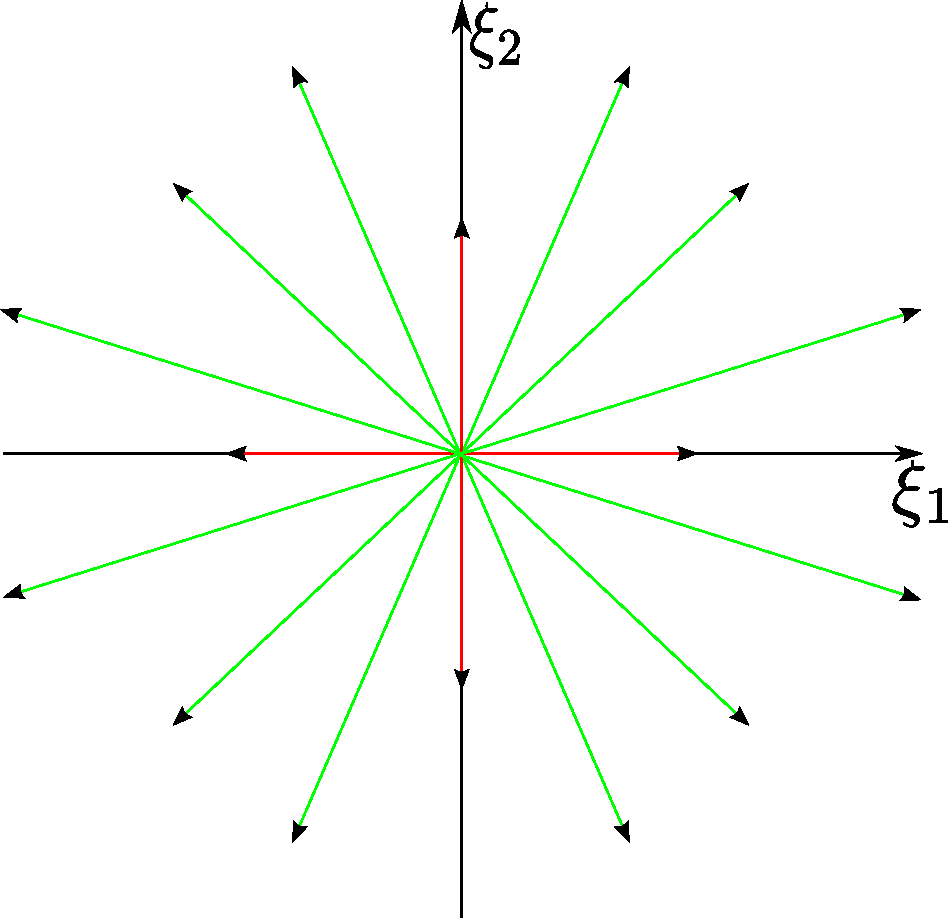
\includegraphics[height=0.20\textheight]{img/lin_sys/lin_sys_3.pdf}
		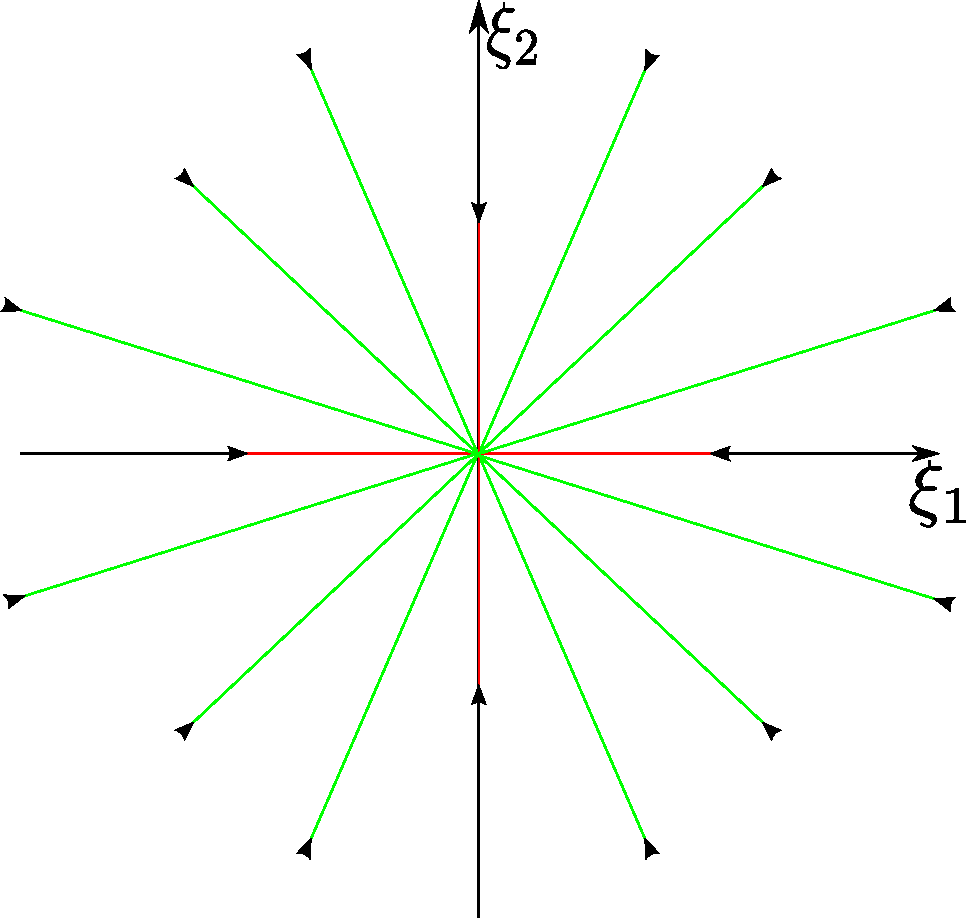
\includegraphics[height=0.20\textheight]{img/lin_sys/lin_sys_4.pdf}
		\caption{3. Fall (links); 4.Fall (rechts)}
	\end{figure}
\subsubsection{5. Fall: \(\lambda_1 < 0 < \lambda_2\)}
					\(x = 0\) wird \emph{Sattelpunkt} genannt und ist offensichtlich instabil. Es ergeben sich in diesem Fall als Orbits Hyperbeln.
		\begin{figure}[htpb]
		\centering
		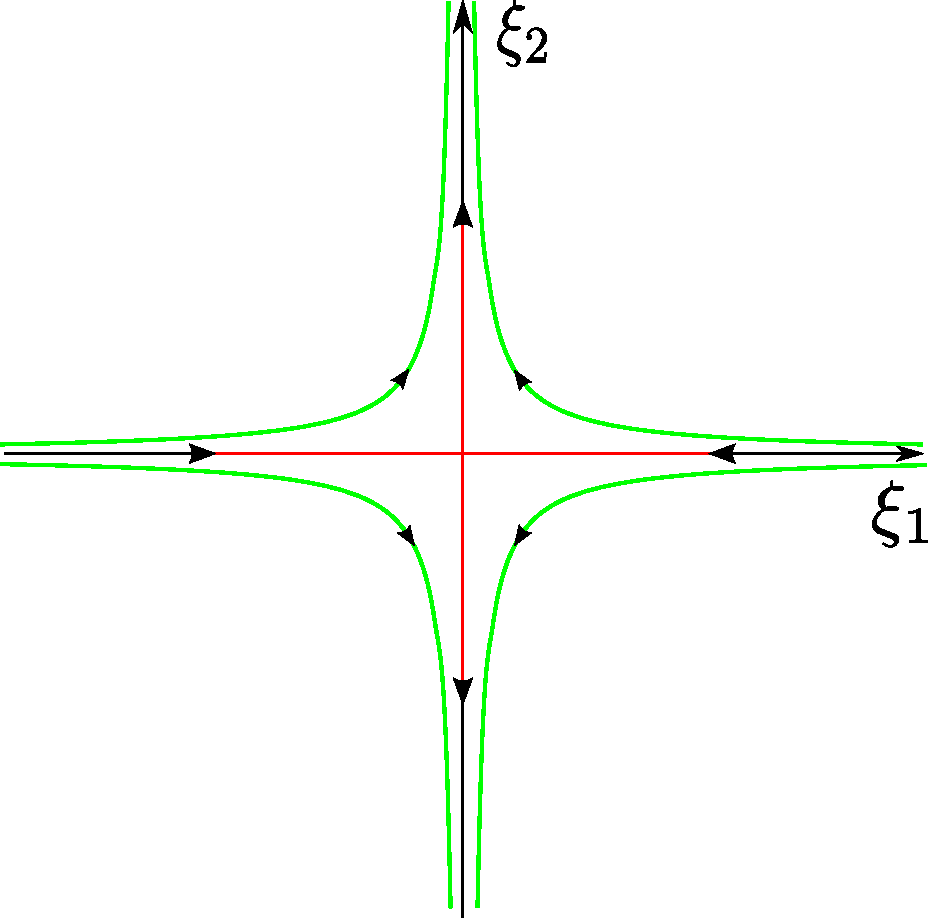
\includegraphics[height=0.20\textheight]{img/lin_sys/lin_sys_5.pdf}
		\caption{5. Fall}
	\end{figure}
	
	
	
	
\subsection{Jordannormalform ist in Pseudo-Diagonalform} 
$A$ habe einen geometrisch einfachen und algebraisch doppelten Eigenwert \({\lambda \in \RR}\). Die Jordannormalform von $A$ ist dann gegeben durch
				$$ J = \left( \begin{array}{cc} \lambda & 1 \\ 0 & \lambda \end{array} \right) $$
Das dazuge"orige Anfangswertproblem lautet
				\[\begin{cases} 
					\dot{\xi_1} = \lambda \xi_1 + \xi_2,\  \xi_1(0) = \xi_{10} \in \RR \\
				 	\dot{\xi_2} = \lambda \xi_2, \qquad\  \xi_2(0) = \xi_{20} \in \RR
				\end{cases} \]
Die L"osungen sind schlie"slich folgenderma"sen gegeben

				$$
				\Rightarrow \xi_2(t) = \xi_{20} e ^{\lambda t} \qquad \Rightarrow \xi_1(t) = \xi_{10} e ^{\lambda t} + t \xi_{20} e ^{\lambda t}$$
				Die Orbits sind analog zur vorherigen Jordannormalform darstellbar als
				$$ \xi_1 = \left( \frac{\xi_{10}}{\xi_{20}} + \frac{1}{\lambda} \ln{\frac{\xi_2}{\xi_{20}}}\right) \xi_2$$
solange keine ung"ultige Rechenoperation durchgef"uhrt wird. 
	\begin{figure}[htpb]
		\centering
		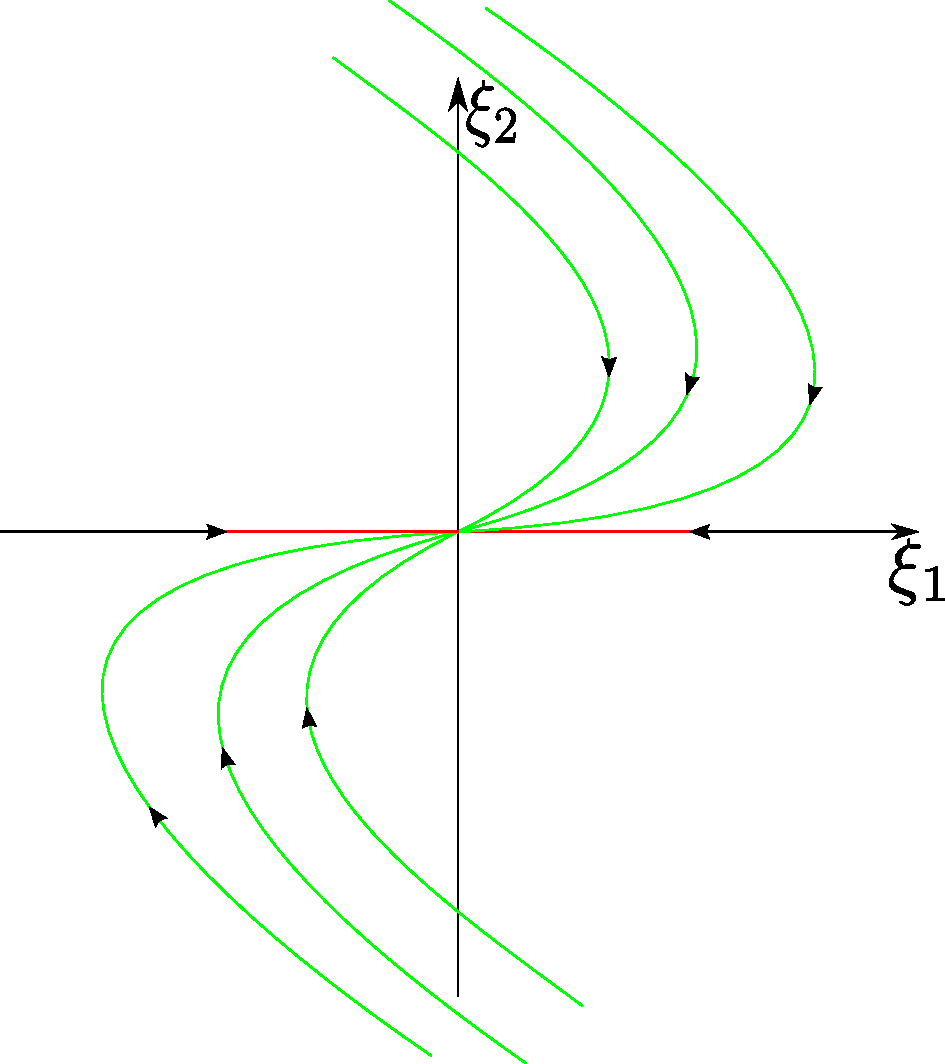
\includegraphics[height=0.31\textheight]{img/lin_sys/lin_sys_6.pdf}
		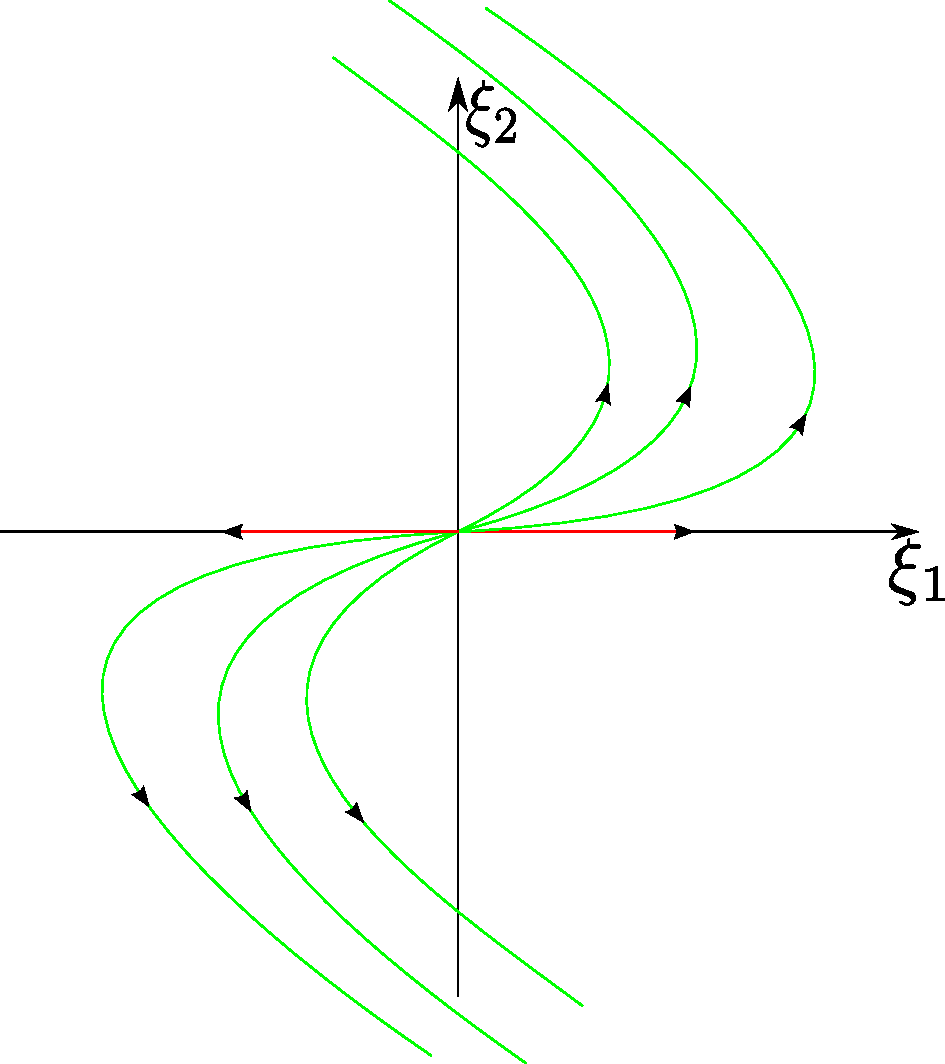
\includegraphics[height=0.31\textheight]{img/lin_sys/lin_sys_6_2.pdf}
		\caption{1. Fall (links); 2.Fall (rechts)}
	\end{figure}
\subsubsection{1. Fall: $\lambda < 0$} 
$x = 0$ wird \emph{stabiler Knoten 3. Art} genannt.
\subsubsection{2. Fall: $\lambda < 0$}
$ x = 0 $ wird \emph{instabiler Knoten 3. Art} genannt.

\subsection{Jordannormalform ist in keiner Diagonalform} 
$A$ habe ein paar komplex konjugierte Eigenwerte $\lambda_{1/2} = \alpha \pm i \beta $. Die reelle Jordannormalform von $A$ ist gegeben durch
				$$ J = \left( \begin{array}{cc} \alpha & \beta \\ - \beta & \alpha \end{array}\right) $$ 
und es ergibt sich das Anfangswertproblem
		\[\begin{cases} 
			\dot{\xi_1} =  \alpha \xi_1 + \beta\xi_2, \ \  \xi_1(0) = \xi_{10} \in \RR \\
			\dot{\xi_2} = -\beta \xi_1 + \alpha \xi_2 , \ \xi_2(0) = \xi_{20} \in \RR
		\end{cases} \]
Die L"osung ist daher		
		\[ \phi(t,\xi_0) = e^{Jt} \xi_0 = e^{(A+B)t} \xi_0 \]
				wobei 
				$$ A = \left( \begin{array}{cc} \alpha & 0 \\ 0 & \alpha \end{array}\right), \ B = \left( \begin{array}{cc} 0 & \beta \\ - \beta & 0 \end{array}\right) $$
Offensichtlich kommutieren $A$ und $B$ miteinander und es gilt $ e^{(A+B)t} = e^{At} e^{Bt} $. Berechnen wir nun die Exponentialmatrix von $A$ bzw. $B$ explizit, so erhalten wir
				$$ e^{At} = e^{\alpha t} \cdot I_2, \  e^{Bt} = \left(\begin{array}{cc} \cos{(\beta t)}  & \sin{(\beta t)} \\ - \sin{(\beta t )} & \cos{(\beta t })  \end{array}\right) \in SO(2) $$
Die explizite L"osung ist dann
				\[\phi(t, \xi_0) = e^{\alpha t} \underbrace{\left(\begin{array}{cc} \cos{(\beta t)}  & \sin{(\beta t)} \\ - \sin{(\beta t )} & \cos{(\beta t })  \end{array}\right)}_{Drehmatrix} \xi_0
				\]
				
\subsubsection{1. Fall: \(\alpha \not = 0\)}
$x=0$ wird \emph{Strudel(Wirbel)} genannt. Falls $\alpha < 0$ so sagt man zus"atzlich, dass $x$ stabil ist. F"ur $\alpha > 0$ entsprechend instabil.
\subsubsection{2. Fall: \(\beta \not = 0\)}
$x=0$ ist \emph{mit den Uhrzeigersinn orientiert}, falls $\beta < 0$. Entsprechend, falls $\beta > 0$ \emph{ gegen den Uhrzeigersinn orientiert}.
\subsubsection{3. Fall: \(\alpha = 0\)}
$x=0$ hei"st \emph{Zentrum}. Dieser ist stabil, jedoch nicht asymptotisch stabil.

\begin{figure}[htpb]
		\centering
		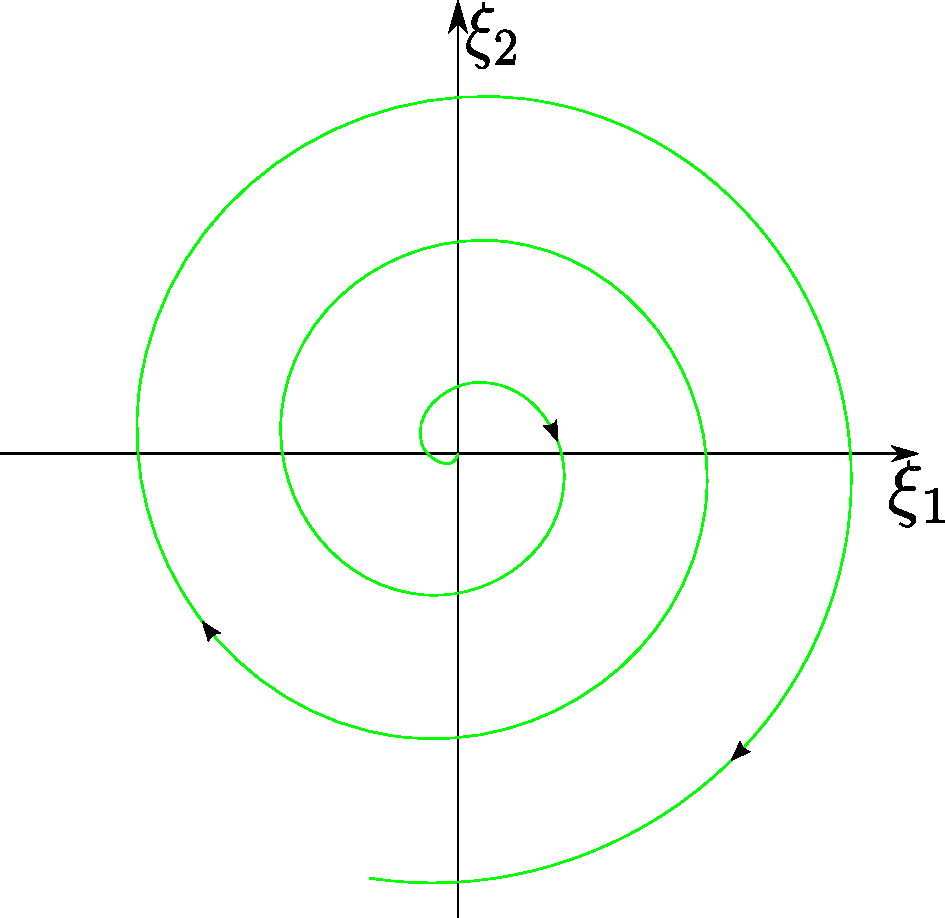
\includegraphics[height=0.25\textheight]{img/lin_sys/lin_sys_7_1.pdf}
		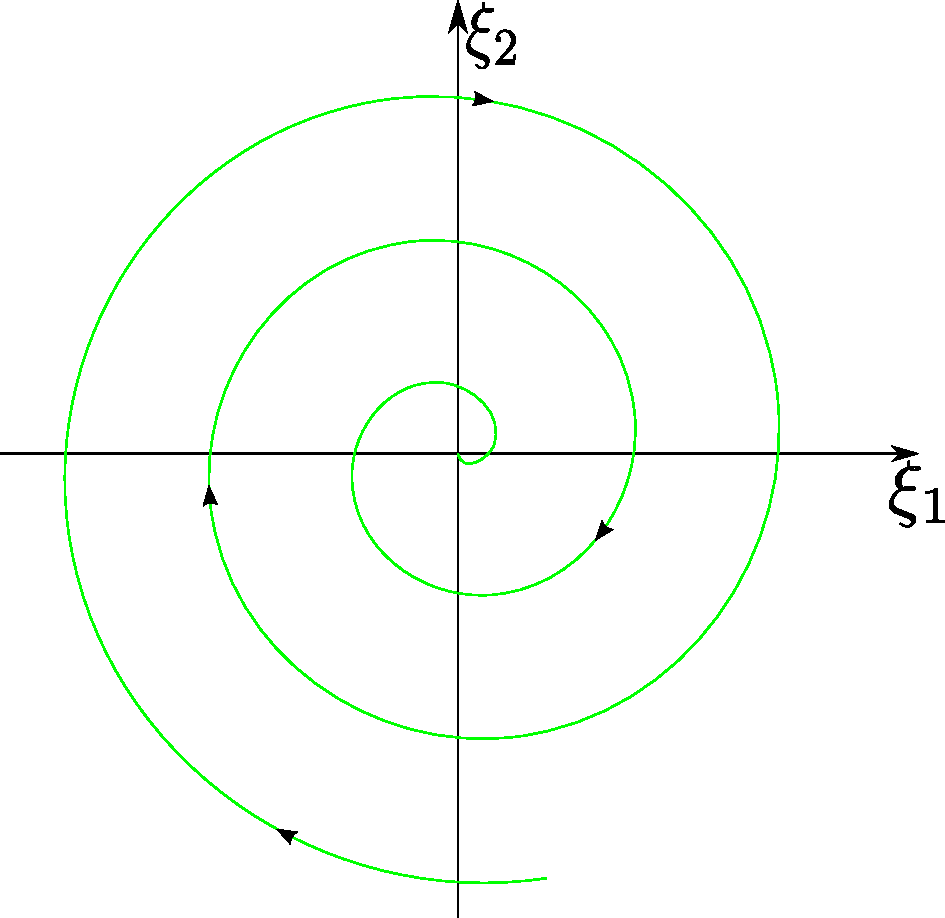
\includegraphics[height=0.25\textheight]{img/lin_sys/lin_sys_7_2.pdf}
		\caption{$\beta < 0 < \alpha$ (links); $\alpha < 0 < \beta$ (rechts)}

		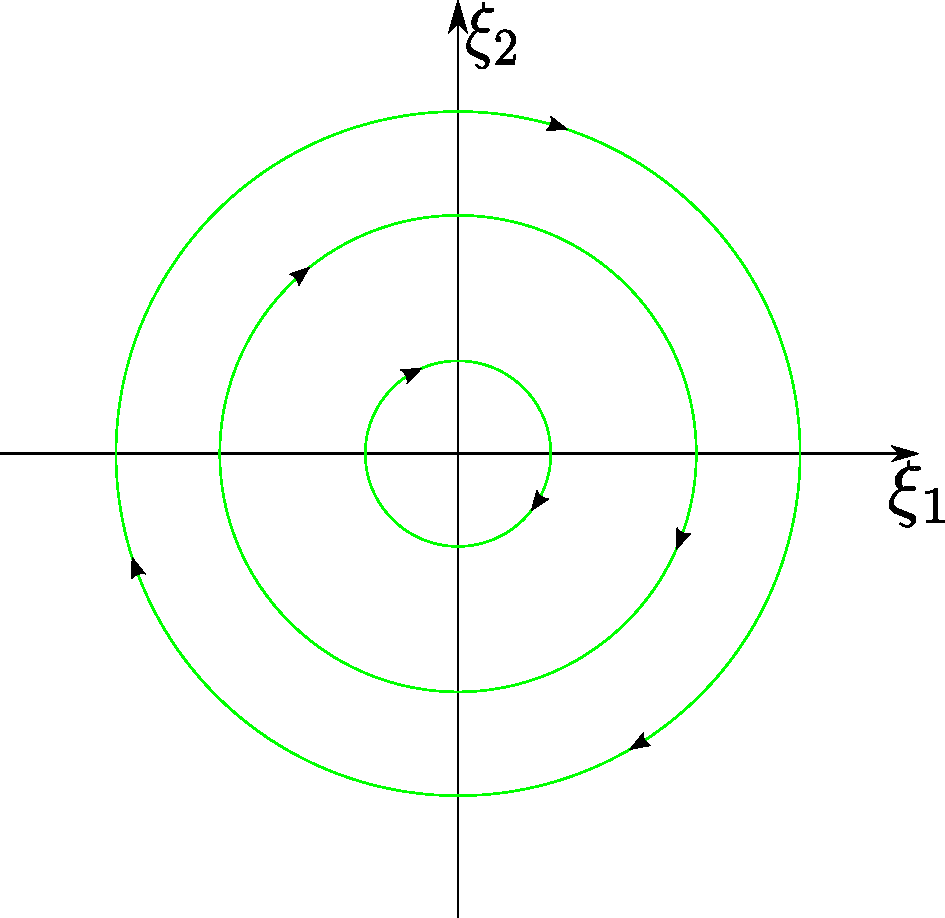
\includegraphics[height=0.25\textheight]{img/lin_sys/lin_sys_7_3.pdf}
		\caption{$\alpha = 0, \beta < 0$}
	\end{figure}
\newpage
\section{Reduktion des Klassifikationsproblems}
\begin{definition}
	Sei \((X,\phi)\) ein dynamisches System. Dann hei"st
	\begin{itemize}
		\item \( M \subset X \) \emph{positiv invariant} \(\Leftrightarrow  \forall t \geq 0: \phi(t,M) \subset M \)
		\item \(\begin{aligned}[t] M \subset X  \text{ \emph{negativ invariant}} 
			& \Leftrightarrow \forall t \leq 0: M \subset \phi(t,M)  \\
			& \Leftrightarrow \forall t \geq 0: \phi(-t,M) \subset M \\
			& \Leftrightarrow \forall t \leq 0: \phi(t,M) \subset M  
			\end{aligned} \)
			
		\item \(\begin{aligned}[t] M \subset X \text{ \emph{invariant}} & \Leftrightarrow M\ \text{positiv und negativ invariant}\\
			& \Leftrightarrow \forall t \in T: \phi(t,M) = M \ 
			\end{aligned} \)
		\end{itemize}	
		Ist \( M \subset X \) invariant, dann bildet 
			\( (M,\left. \phi(t,\cdot)\right|_M) \) ein dynamisches System auf M und wird \emph{Teilsystem} des urspr"unglichen Systems \((X,\phi)\) genannt. 	
\end{definition}

\begin{description}
\item [Bemerkung]
	Jeder invariante Untervektorraum \(U \subset \RR^n \) bzgl. der linearen Abbildung 
		\[x \mapsto Ax : \RR^n \rightarrow \RR^n \]
(d.h. $x\in U\Rightarrow Ax \in U$ ) ist ein invarianter Untervektorraum des GDG-Systems \(\dot{x} = Ax\), denn
		\[\phi(t,x_0) = e^{At} x_0 = \sum_{j=0}^{\infty} \frac{t^j}{j!} \underbrace{A^j x_0}_{\in U}, \qquad x_0 \in U\]
Der Wert der Summe liegt in \(U\), da $U$ abgeschlossen und sie Grenzwert ist von
	\[ e^{At} x_0 = \lim_{N\to \infty} \underbrace{\sum_{j=0}^{N} \frac{t^j}{j!} A^j x_0 }_{\in\  U\ \forall N} \]
\end{description}

\begin{corollar}
	Alle Eigenr"ame \(E_j\) (bzw. verallgemeinerte Eigenr"aume), sowie deren direkte Summen sind kanonisch invariante Unervektorr"aume des Systems
		\[\dot{x} = Ax, \qquad A \in \RR^{n\times n} \]
	\underline{Speziell:} Ist \(\RR^n = \oplus_{j=1}^{N} E_j \) eine direkte Summe von (relativ niedrig dimensionierten) Eigenr"aumen von \(A\), dann ist das urspr"ungliche System \(\dot{x}=Ax\) das direkte Produkt der Teilsysteme auf den \(E_j\).
	Falls sich die Teilsysteme vollst"andig analysieren bzw. klassifizieren lassen, dann auch das urspr"ungliche System \(\dot{x} = Ax\) im \(\RR^n\)
\end{corollar}

\begin{definition}
	Spezielle (verallgemeinerte) Eigenr"aume von \(A\) und damit invariante Untervektorr"aume von \(\dot{x}=Ax\) : 
	\begin{itemize} 
		\item stabiler Unterraum von \(\dot{x}=Ax\)
			$$E^s := \left\{\left. v\in \RR^n \right| (A-\lambda \operatorname{id})(v) = 0 \land \operatorname{Re}(\lambda) < 0\right\}$$ 
			Dies ist der verallgemeinterte Eigenraum zu allen Eigenwerten $\lambda$ von $A$ mit $\operatorname{Re}\lambda < 0$.
		\item instabiler Unterraum von \(\dot{x}=Ax\)
		$$E^u := \left\{\left. v\in \RR^n \right| (A-\lambda \operatorname{id})(v) = 0 \land \operatorname{Re}(\lambda) > 0\right\}$$ 
			Dies ist der verallgemeinterte Eigenraum zu allen Eigenwerten $\lambda$ von $A$ mit $\operatorname{Re}\lambda > 0$.
		\item Zentrums-Unterraum von \(\dot{x}=Ax\)
		$$E^c := \left\{\left. v\in \RR^n \right| (A-\lambda \operatorname{id})(v) = 0 \land \operatorname{Re}(\lambda) = 0\right\}$$ 
			Dies ist der verallgemeinterte Eigenraum zu allen Eigenwerten $\lambda$ von $A$ mit $\operatorname{Re}\lambda = 0$.
	\end{itemize}
\end{definition}
\begin{figure}[htpb]
		\centering
		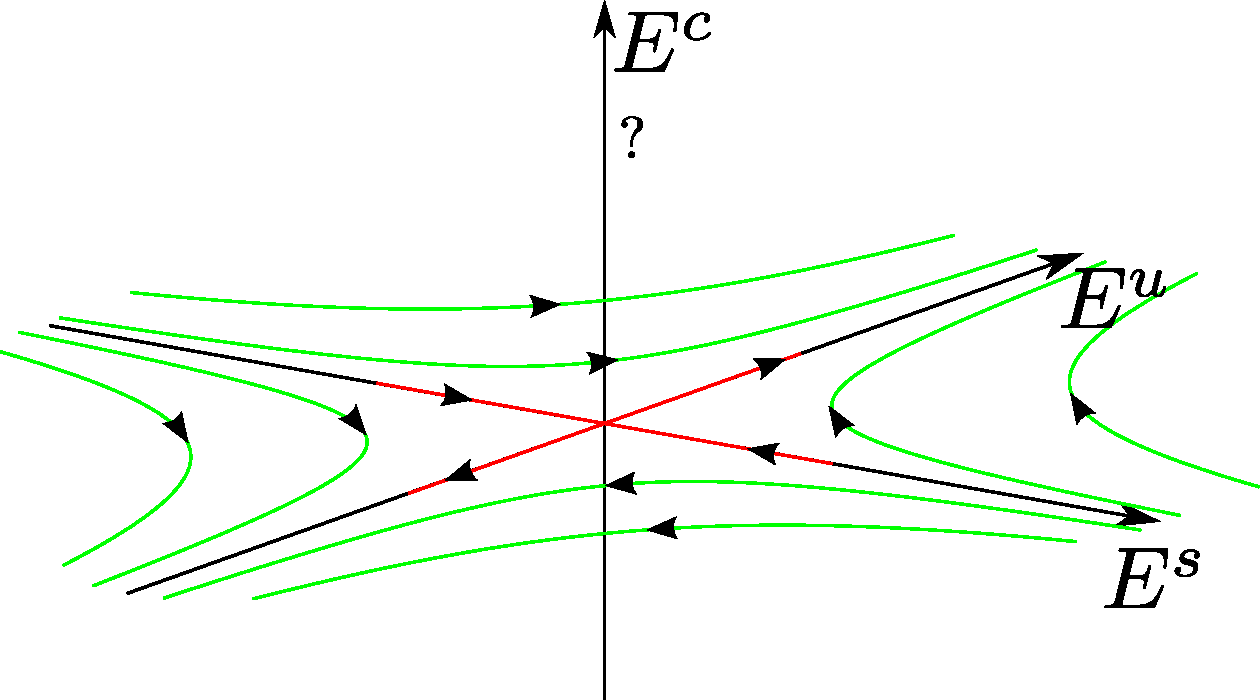
\includegraphics[height=0.30\textheight]{img/eigenraeume.pdf}
		\caption{$E^c$ entscheidet viel "uber das Verhalten der Orbits}
\end{figure}

\begin{satz}
Es gilt: 
	\[\RR^n = E^s \oplus E^u \oplus E^c \]
\end{satz}

\begin{description}
	\item[Terminologie]Spezielle Eigenraum-Typen des GDG-Systems $\dot x = Ax$ \\
	\begin{itemize}
		\item \(E^c = \{0\} \Rightarrow x =0\) hei"st hyperbolischer Gleichgewichtspunkt 
		\item \(E^c = \{0\}, {E^s \not= \{0\}, E^u \not= \{0\}} \Rightarrow x =0\) hei"st Sattelpunkt
		\item \(E^c = \{0\}, E^u = \{0\} \Rightarrow x =0\) hei"st Senke (asympt. stabil) 
		\item \(E^c = \{0\}, E^s = \{0\} \Rightarrow x =0\) hei"st Quelle (instabil)
		
	\end{itemize}
\end{description} 

\section{Klassifikation von Phasendiagrammen von Hom-Systemen f"ur $n=1$}

Sei $X = \RR, \ \psi\colon X \to X$ ein linearer Hom"omorphismus, der das lineare dynamische Systeme $(X,\phi)$ erzeugt. Insbesondere ist $\psi(x) = ax$ f"ur ein $a\in\RR\setminus\{0\}$.

Man kann dann die Orbits folgenderma"sen klassifizieren.
\subsubsection{Falls $|a| < 1$}
$x=0$ wird \emph{Senke} genannt und ist stabil.
\subsubsection{Falls $|a| > 1$}
$x=0$ wird \emph{Quelle} genannt und ist instabil.
\subsubsection{Falls $ a < 0$}
$x=0$ wird \emph{orientierungsumkehrend} genannt.
\subsubsection{Falls $a > 0$}
$x=0$ wird \emph{orientierungserhaltend} genannt.
\subsubsection{Falls $|a| = 1$}
$x=0$ wird \emph{Zentrum} genannt. Ist $a = 1$, so ist jeder Punkt $x\in\RR$ ein Gleichgewichtspunkt. F"ur $a=-1$ ergeben sich 2-periodische Orbits (gez"ahlt an der minimalen positiven Periode).

\begin{figure}[htpb]
		\centering
		\includegraphics[width=1\textwidth]{img/lin_sys/diskret/lin_sys_1.pdf}
		\caption{$|a| < 1, \ a < 0$}

		\includegraphics[width=1\textwidth]{img/lin_sys/diskret/lin_sys_2.pdf}
		\caption{$|a| > 1, \ a > 1$}

		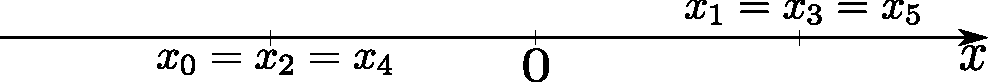
\includegraphics[width=1\textwidth]{img/lin_sys/diskret/lin_sys_3.pdf}
		\caption{$a = -1$}
\end{figure}

\begin{description}
\item[Bemerkung]
	Jeder der bzgl. der linearen Abbildung \(x\mapsto Ax \) invarianter Unterverktorraum \(U\) ist invariant bzgl. des von \(\psi(x) = Ax \) erzeugten dynamische Systems.
\end{description}

%-----------------------------------------------------------------------------------------------

\chapter{Grobman-Hartman-Theorem}

\section{Kontinuierlicher Fall}
Sei $(X,\phi)$ ein dynamisches System, das durch die Differentialgleichung ${\dot x = v(x)}$ induziert ist, wobei $v \in C^k(\RR^n, \RR^n), \ k \geq 1$. Sei zus"atzlich  $x_G$ ein Gleichgewichtspunkt des dynamischen Systems. Betrachte die \emph{Linearisierung} des Systems um $x_G$ 
\[\dot{\xi}=Jv(x_G)\xi, \ \xi =x-x_G\] 
( $\dot{\xi}(x_G)\approx v(x)$, falls $\Vert\xi\Vert\ll 1$ )

\begin{satz}[Grobman-Hartman]\label{Grobman-Hartman}
Gegeben sei ein dynamisches System $(X,\phi)$ wie oben, wobei $x_G$ ein hyperbolischer Gleichgewichtspunkt ist, d.h. $\operatorname{Re}\lambda \neq 0$ f"ur alle Eigenwerte $\lambda$ von $Jv(x_G)$. Dann existiert eine Umgebung $U\subseteq \RR^n$ von $\xi =0$ und ein Hom"oomorphismus $h:U\to\mathbb{R}^n$, so dass \[ \forall t\in D: h(e^{Jv(x_G)t}\xi)=\phi(t,h(\xi))\ \] wobei $D := \left \{ \left . t \in \RR \right| e^{Jv(x_G)t}\xi \in U \right \}$ bezeichne.
\end{satz}
\begin{figure}[htpb]
		\centering
		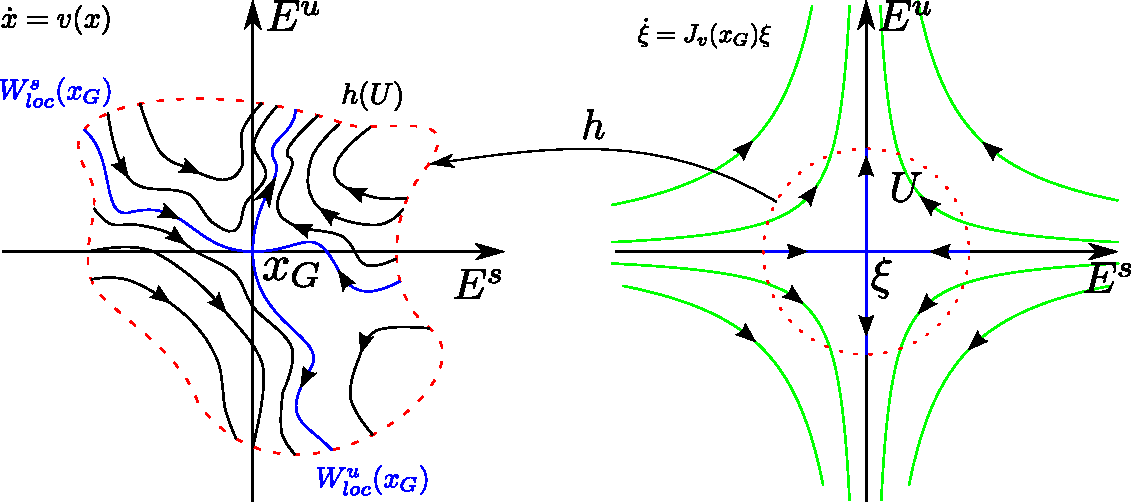
\includegraphics[width=1\textwidth]{img/grobman-hartman.pdf}
		\caption{Illustration Grobman-Hartman-Theorem}
\end{figure}

Somit bildet $h$ hom"oomorph die Orbits des linearisierten Systems durch $\xi\in U$ auf diejenigen des nichtlinearen Systems durch $h(\xi)$ ab, wobei die zeitliche Orientierung erhalten bleibt. Man sagt, die beiden Systeme sind mittels des Hom"oomorphismus \emph{topologisch konjugiert} zueinander. Insbesondere ist damit also das lokale Phasenportrait des nichtlinearen Systems nahe $x_G$ ein hom"oomorphes Abbild des lokalen Phasenportraits des linearisierten Systems in U; die Bezeichnung zur Typisierung (Klassifikation) entsprechender hyperbolischer Gleichgewichtspunkte nichtlinearer Systeme "ubernimmt man vom linearen Fall, z.B: Ist $\xi =0$ ein Sattelpunkt von $\dot{\xi}=Jv(x_G)\xi$, dann ist auch $x_G$ ein Sattelpunkt von $\dot{x}=v(x)$.

\begin{description}
\item[Bezeichnung]Wir f"uhren folgende Bezeichnungen ein
\begin{itemize}
\item $h(E^s\cap U)=: W_{loc}^s(x_G)$ lokale stabile Mannigfaltigkeit von $x_G$ (positiv invariant)\\
\item $h(E^u\cap U)=: W_{loc}^u(x_G)$ lokale instabile Mannigfaltigkeit von $x_G$ (negativ invariant)\\
\item $W^s(x_G):=\{x\in\mathbb{R}^n|\lim\limits_{t\to +\infty}\phi (t,x)=x_G\}$ hei"st (globale) stabile Mannigfaltigkeit von $x_G$\\
\item $W^u(x_G):=\{x\in\mathbb{R}^n|\lim\limits_{t\to -\infty}\phi (t,x)=x_G\}$ hei"st (globale) instabile Mannigfaltigkeit von $x_G$
\end{itemize}
\end{description}

\begin{bemerkung}
$W^s(x_G)$ und $W^u(x_G)$ sind invariant, d.h.
\begin{align*}
\phi(t,W^{s/u}(x_G))=W^{s/u}(x_G)\ \forall t\in\mathbb{R} \\
x\in W^s(x_G)\ \Rightarrow\ \lim_{t\to\infty}\phi(t,x)=x_G\\
\Rightarrow\ \lim_{t\to\infty}\phi(t,\phi(s,x))=\lim_{t\to\infty}\phi(t+s,x)=x_G \text{ f"ur jedes }  s\in\mathbb{R}\\
\Rightarrow\ \phi(s,x)\in W^s(x_G)\\
\Rightarrow\ \phi(s,W^s(x_G))=W^s(x_G)\ \forall s\in\mathbb{R}
\end{align*}
\end{bemerkung}

\begin{satz}["Uber die lokalen stabilen und instabilen Mannigfaltigkeiten eines hyperbolischen Gleichgewichtspunktes]
Unter den Voraussetzungen von \eqref{Grobman-Hartman} gibt es eine Umgebung $U\subseteq \RR^n$ von $x_G$, sodass  Abbildungen
\[h^s:E^s\cap V\to E^u \text{ und } h^u:E^u\cap V\to E^s\]
existieren, die so glatt sind wie das Vektorfeld $v(x)$, so dass
\[W_{loc}^s(x_G)=\operatorname{graph}(h^s, E^s\cap V) \]und
\[W_{loc}^u(x_G)=\operatorname{graph}(h^u, E^u\cap V) \]
mit $h^{s/u}(x_G)=0$ und $J_{h^{s/u}}(x_G)=0$, d.h. $W_{loc}^{s/u}(x_G)$ ist in $x_G$ tangential zu $E^{s/u}$. Speziell kann $V = h(U)$ gew"ahlt werden, wobei $h$ der Hom"oomorphismus aus \eqref{Grobman-Hartman} ist.
\end{satz}

\begin{beispiel}
Gegeben sei folgende Differentialgleichung
\begin{align*}
v( \begin{pmatrix} x \\ y\end{pmatrix} ) = \begin{cases}
&\dot{x}=x\\
&\dot{y}=-y+x^2
\end{cases}
\end{align*}
Ein Gleichgewichtpunkt ist $x_G=(0,0)$. Die Jacobi-Matrix erf"ullt in $x_G$ 
\[Jv(x_G)=\begin{pmatrix} 1&0\\ 0&1 \end{pmatrix}\]
Daher sind die Eigenwerte 
\[ \lambda_1=-1, \lambda_2=1\\
\Rightarrow\ x_G  \text{ hyperbolischer Sattelpunkt}\]
und der Satz von Grobman-Hartman ist anwendbar. Die Orbitgleichung erh"alt man folgenderma"sen:
\begin{align*}
\frac{dy}{dx}=\frac{\frac{dy}{dt}}{\frac{dx}{dt}}=\frac{-y+x^2}{x} \text{ (f"ur $x\neq 0$) } =-\frac 1 x \cdot y+x\\
\Rightarrow\ y(x)=\frac 1 3 x^2+\frac c x, c\in\mathbb{R} \text{ beliebig} \\
\Rightarrow\ h^u:\mathbb{R}\to\mathbb{R}, x\mapsto\frac{x^2} 3\ (c=0)\\
\Rightarrow\ h^u(0)=0, (h^u)'(0)=Jh^u(0)=0\\
h^s:\mathbb{R}\to\mathbb{R}, x\mapsto 0
\end{align*}
\end{beispiel}


\section{Diskreter Fall}
Sei $\psi$ ein $C^k$-Diffeomorphismus von $\mathbb{R}^n$ nach $\mathbb{R}^n$, d.h. $\psi$ ist bijektiv und $\psi^{-1}\in C^k(\mathbb{R}^{n},\mathbb{R}^{n})$, $x_G$ ein Gleichgewichtspunkt des von $\psi$ erzeugten dynamischen Systems. Betrachte die Linearisierung dieses Systems in $x_G$, erzeugt durch $J\psi(x_G)$ (regul"ar). ($\psi(x)\approx J\psi(x_G)\xi, \xi=x-x_G, \Vert\xi\Vert\ll 1$)

\begin{satz}[Grobman-Hartman]
Unter diesen Voraussetzungen existiert eine Umgebung $0\in U\subset \mathbb{R}^n$ und ein Hom"oomorphismus $h:U\to h(U)\subset\mathbb{R}^n, h(0)=x_G$, sodass das von $J\psi(x_G)\xi$ erzeugte System bzgl. $h$ lokal topologisch konjugiert ist, d.h.
\begin{align*}
h(J\psi(x_G)\xi)=\psi(h(\xi)), \xi\in U\\
h(J\psi(x_G)^k\xi)=\psi^k(h(\xi)), k\in\mathbb{Z} \text{ beliebig}
\end{align*}
sofern $x_G$ ein hyperbolischer Gleichgewichtspunkt des $\psi$-Systems ist, d.h. $\xi=0$ ein hyperbolischer Gleichgewichtspunkt des linearisierten $J\psi(x_G)$-Systems ist.
\end{satz}

Die restliche Grobman-Hartman-Theorie ist analog zum kontinuierlichen Fall.

\begin{beispiel}
$\psi(x)=x^3$ erzeugender Hom"oomorphismus ($C^k$-Diffeomorphismus f"ur $1\leq k\leq\infty$ au"serhalb von $x=0$)\\
Als Voraussetzung der Grobman-Hartman-Theorie gen"ugt es, wenn die Voraussetzungen lokal nahe der betrachteten Gleichgewichtspunkte erf"ullt sind.
\[x_G=\pm 1, J\psi(x_G)=3>1\ \Rightarrow\ x_G\text{ orientierungserhaltende Quelle}\]
Gesucht ist ein Hom"oomorphismus $h$, welcher das $\psi$- und das $J\psi(x_G)$-System lokal nahe $x_G=\pm 1$ konjugiert (in $U_1=(-\infty, 0), U_2=(0,+\infty)$).\\
$h:\mathbb{R}\to\mathbb{R}, \xi\mapsto h(\xi)$ stetig, bijektiv, sodass
\begin{align*}
h(3\xi)=h(\xi)^3\ \forall\xi\in U\\
\Leftrightarrow \ln h(3\xi)=3\ln h(\xi)\\
\Rightarrow\ \ln\circ h(\xi)=\xi\\
\Rightarrow\ h(\xi)=e^{\xi}, h(0)=1 \text{ in } U_2=(0,+\infty)
\end{align*}
\end{beispiel}

\chapter{Periodische Orbits}
\section{Begriff und Bestimmung von periodischen Orbits}
\begin{definition}
Sei $(X,\phi)$ ein dynamisches System. Ein Orbit $\Gamma_{x_p} = \left \{ \left. \phi(t, x_p) \right | t \in \RR \right \}$ hei"st $T$-periodisch, falls $T>0$ und 
$$\forall t \in \RR: \phi(t, x_p) = \phi(t + T, x_p)$$
Das minimale $T>0$ hei"st \emph{Periode} des Orbits $\Gamma_{x_p}$. $x_p$ nennt man $T$-periodischen Punkt des Systems.
\end{definition}
\begin{figure}[htpb]
		\centering
		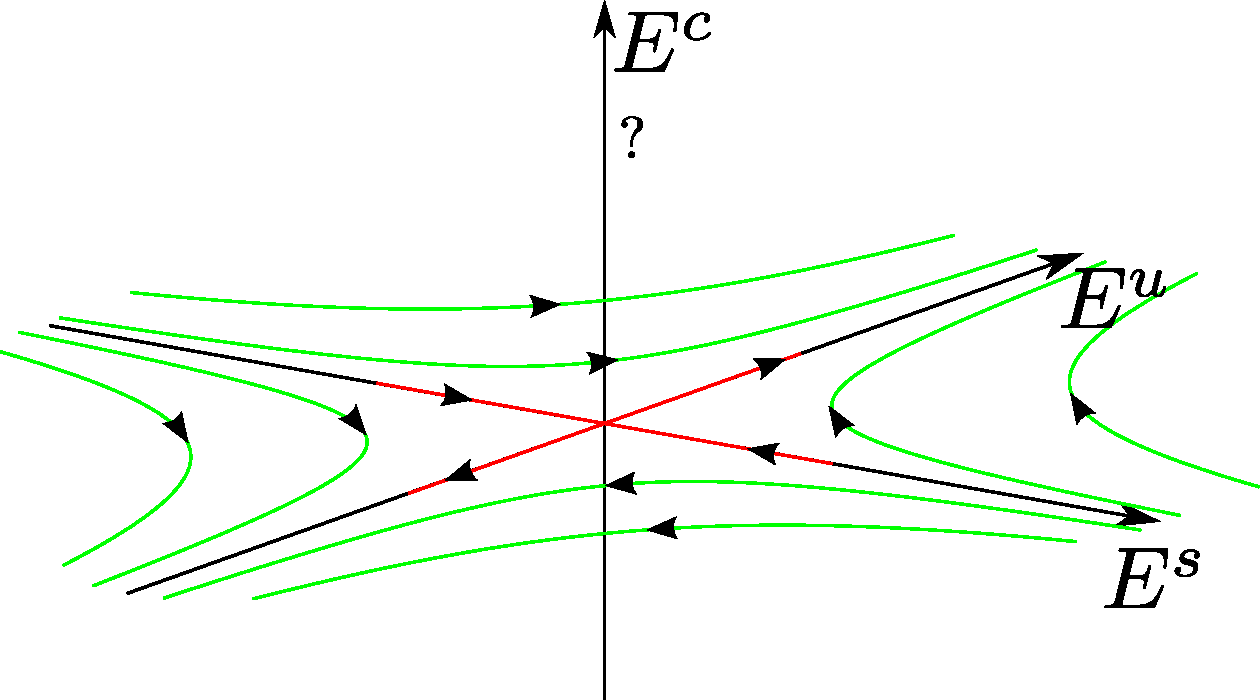
\includegraphics[width=0.8\textwidth]{img/periodische_orbits/disk_kont.pdf}
		\caption{periodische Orbits}
\end{figure}

\begin{description}
\item[Bemerkung]
Falls $x_p$ ein $T$-periodischer Punkt ist, so ist auch jeder andere Punkt $x\in \Gamma_{x_p}$ $T$-periodisch.
\end{description}
\subsection{Bestimmungsgleichung f"ur periodische Punkte}
Die Bestimmungsgleichung ist folgenderma"sen gegeben
$$\phi(T, x_p) = \phi(0, x_p)$$
f"ur ein minimales $T > 0$. Speziell im diskreten Fall ergibt sich
$$\phi(T, x_p) = \psi^T(x_p) = x_p$$

\begin{beispiel}
$\psi(x) = -x , \ x \in \RR$. 
Bestimmungsgleichung f"ur $2$-periodische Punkte
$$\psi^2(x_p) = \operatorname{id}(x_p) = x_p$$
Folglich ist jeder Punkt $x_p\in\RR\setminus\{0\}$ ein $2$-periodischer Punkt, also gilt ${\Gamma_{x_p} = \left \{ x_p, -x_p\right\}}$. F"ur $x = 0$ liegt ein Gleichgewichtspunkt vor (man sagt auch $1$-periodisch). 
\begin{figure}[htpb]
		\centering
		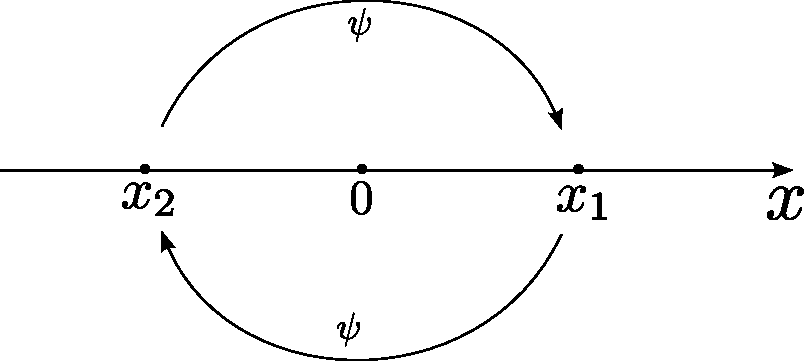
\includegraphics[width=0.7\textwidth]{img/periodische_orbits/beispiel_per_orbit.pdf}
		\caption{periodische Orbits}
\end{figure}
\end{beispiel}
\section{Poincar\'{e}  Abbildung f"ur GDG-Systeme}
Sei $(X,\phi)$ ein dynamisches System, das durch die Differentialgleichung $\dot x = v(x), \ x \in \RR^n$ erzeugt wird.
\begin{definition}
Sei $x_p$ ein $T$-periodischer Punkt. Es existiert ein $n\in\RR^n$, sodass $\langle v(x_p), n \rangle \neq 0$, beispielsweise $n = v(x_p)$. Die $(n-1)$-dimensionale Untermannigfaltigkeit
$$\Sigma_{x_p} := \left \{ \left. x \in X \right| \langle x - x_p, n \rangle =0 \right \}$$ 
schneidet den Orbit $\Gamma_{x_p}$ \emph{transversal} in $x_p$ und wird auch \emph{Poincar\'{e} Schnitt} genannt. Sei $V\subseteq \RR^n$ eine hinreichend kleine Umgebung von $x_p$. Die \emph{erste R"uckkehrzeit} $\tau\colon \Sigma_{x_p} \cap V \to \RR$ ist definiert als
$$\tau(x) := \min \left \{ \left. t> 0 \right| \phi(t, x) \in \Sigma_{x_p} \cap B_{\varepsilon(x)}(x) \right \}$$
wobei $\varepsilon(x)$ hinreichend klein gew"ahlt ist.
\end{definition}
\begin{description}
\item[Bemerkung] 
Die erste R"uckkehrzeit gibt die Zeit an, die ben"otigt wird um, ausgehend vom Punkt $x \in \Sigma_{x_p}\cap V$, die transversale Menge $\Sigma_{x_p}$ nach einem vollen Umlauf wieder zu schneiden. Das hei"st es gilt $\phi(\tau(x), x) \in \Sigma_{x_p}$, sowie $\tau(x_p) = T$ nach Definition.
\end{description}
\begin{figure}[htpb]
		\centering
		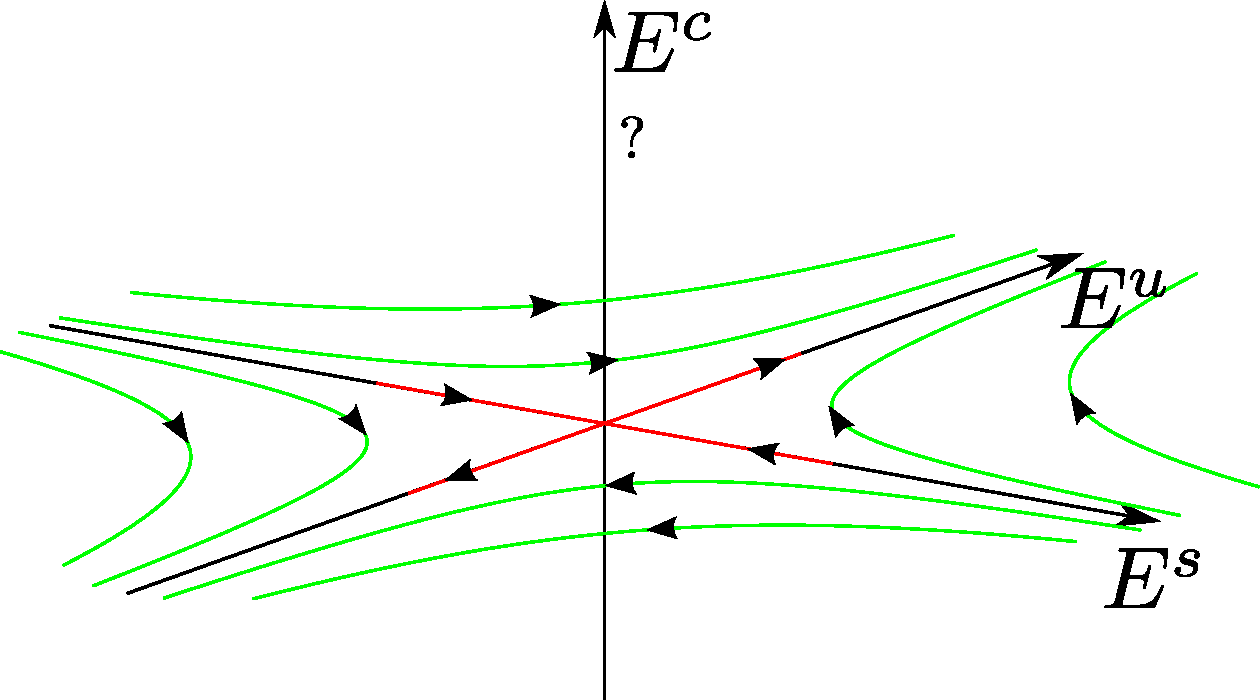
\includegraphics[width=0.5\textwidth]{img/periodische_orbits/transversal_rueckkehrzeit.pdf}
		\caption{Transversale Menge $\Sigma_{x_p}$, sowie erste R"uckkehrzeit}
\end{figure}
\begin{lemma}\label{rueckkehrzeit_diffbar}
Sei $v \in C^k(\RR^n,\RR^n)$ ein Vektorfeld mit $k \in \mathbb{N}$. Dann existiert eine Umgebung $V\subseteq \RR^n$ von $x_p$, sodass $\tau \in C^k(V, \RR)$.
\end{lemma}
\begin{beweis}
Definiere Funktion $F \colon \RR \times \RR^n \to \RR, \ (t, x) \mapsto \langle \phi(t, x) - x_p, n\rangle$. F ist $k$-fach stetig differenzierbar. Wir weisen die Voraussetzungen f"ur den Satz von der impliziten Funktion nach
\begin{itemize}
	\item Es gilt $F(T, x_p) = 0$ 
	\item Die Ableitung von $F$ nach $t$ ist invertierbar in $x_p$
	\begin{align*}
		&\frac{\mathrm d}{\mathrm dt} \langle \phi(t, x) - x_p, n\rangle =  \langle \frac{\mathrm d}{\mathrm dt} \phi(t, x), n\rangle = \langle v(x), n \rangle\\
		&\Rightarrow \left. \frac{\mathrm d}{\mathrm dt} \langle \phi(t, x) - x_p, n\rangle \right|_{x=x_p} = \langle v(x_p), n \rangle \neq 0
	\end{align*}
\end{itemize}
Der Satz von der impliziten Funktion anwendbar und es existiert daher ein $V\subseteq \RR$, sowie $f \in C^k(V, \RR)$, sodass gilt
\begin{enumerate}
	\item $f(x_p) = T$
	\item $\forall x \in V: F(f(x), x) = 0$
\end{enumerate}
Dieses $f$ stellt die erste R"uckkehrzeit $\tau$ dar, denn es gilt
$$ F(\tau(x), x) = \langle \phi(\tau(x), x) - x_p, n\rangle = 0 = F(f(x), x) $$
\qed
\end{beweis}
\begin{definition}
Die Abbildung
$$P_{\Sigma_{x_p}} \colon V \cap \Sigma_{x_p} \to \Sigma_{x_p},\ x\mapsto \phi(\tau(x), x)$$
hei"st \emph{Poincar\'{e} Abbildung (des periodischen Orbits $\Gamma_{x_p}$ bez"uglich $\Sigma_{x_p}$)}. 
\end{definition}
\begin{description}
\item[Bemerkung] Falls $v\in C^k$, so ist $P_{\Sigma_{x_p}} \in C^k$. Dies ist eine direkte Folgerung von \eqref{rueckkehrzeit_diffbar}, sowie der Eigenschaft, dass $\phi \in C^k$. Die Poincar\'{e} Abbildung besitzt einen Fixpunkt, denn ${P_{\Sigma_{x_p}}(x_p) = x_p}$. Allgemeiner gilt folgendes Lemma 
\end{description}

\begin{lemma}
Sei $x$ ein Fixpunkt von $P_{\Sigma_{x_p}}^N$ mit einem minimalen $N \in \mathbb{N}$. Dann ist $\Gamma_x$ ein periodischer Orbit mit Periode
$$ \sum_{j=1}^N{\tau(x_j)}$$
wobei $x_1 = x, \ x_{j+1} = \phi(\tau(x_j), x_{j})$ f"ur $j = 1,\ldots N$ \
\end{lemma}
\section{Stabilit"atsanalyse periodischer Orbits mittels Poincar\'{e} Abbildung}
\begin{definition}[Orbitale dynamische Stabilit"at]
Sei $(X,d)$ ein metrischer Raum, $(X,\phi)$ ein dynamisches System mit einem periodischen Orbit $\Gamma_{x_p}$. Dann hei"st $\Gamma_{x_p}$ 
\begin{itemize}
\item \emph{orbital stabil}, falls 
	$$ \forall \varepsilon > 0 \exists \delta > 0 \forall x\in X, t\geq 0:
	\operatorname{dist}(x, \Gamma_{x_p}) < \delta \Rightarrow \operatorname{dist}(\phi(t,x), \Gamma_{x_p}) < \varepsilon$$
\item \emph{orbital instabil }, falls $\Gamma_{x_p}$ nicht orbital stabil ist.
\item \emph{orbital asymptotisch stabil}, falls $\Gamma_{x_p}$ orbial stabil ist und gilt
$$ \exists b > 0 \forall x \in X: \operatorname{dist}(x, \Gamma_{x_p}) < b \Rightarrow \lim_{t\to\infty}{\operatorname{dist}(\phi(t,x), \Gamma_{x_p})} = 0 $$
\end{itemize}
wobei $\operatorname{dist}(x, M) := \inf_{y\in M}{d(x,y)}, \ M\subseteq X$. Zu orbital asymptotisch stabilen Orbits $\Gamma_{x_p}$ sagt man auch \emph{Grenzzykel}.
\end{definition}
\begin{figure}[htpb]
		\centering
		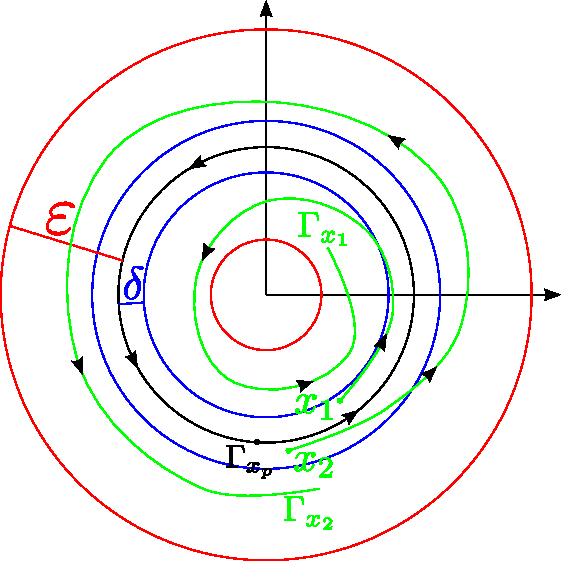
\includegraphics[width=0.4\textwidth]{img/periodische_orbits/orbiale_stabilitaet.pdf}
		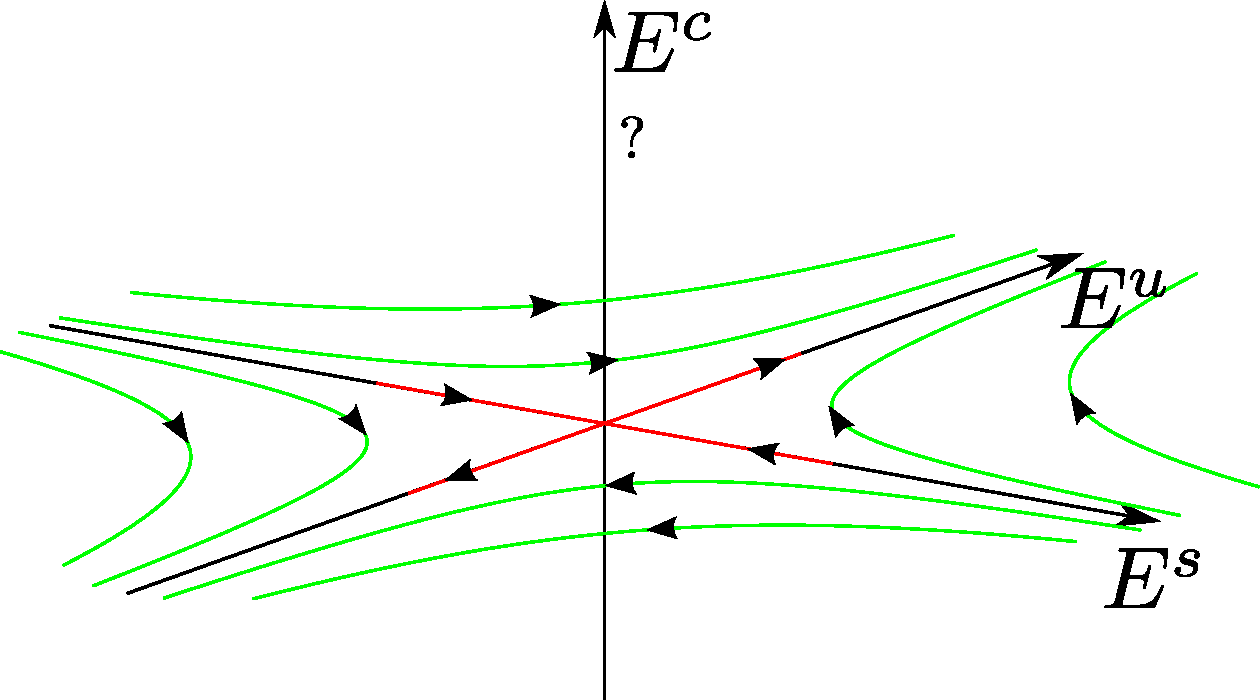
\includegraphics[width=0.4\textwidth]{img/periodische_orbits/orbitale_asymp_stabilitaet.pdf}
		\caption{Orbitale Stabilit"at(links); Orbitale asymptotische Stabilit"at (rechts)}
\end{figure}
\begin{satz}[Stabilit"atskriterium]\label{stabilitatskriterium_periodische_orbits}
Sei $\Gamma_{x_p}$ ein periodischer Orbit von $(X, \phi)$, $\Sigma_{x_p}$ ein Poincar\'{e} Schnitt durch $x_p$ und $P_{\Sigma_{x_p}}$ eine zugeh"orige Poincar\'{e} Abbildung. Es existiert eine Umgebung $V\subseteq \RR^n$ von $x_p$, sodass $(\Sigma_{x_p}\cap V, \psi)$ ein diskretes dynamisches System durch $\psi(n, x) := P_{\Sigma_{x_p}}^n(x)$ induziert, das den Gleichgewichtspunkt $x_p$ besitzt. 
Dann sind "aquivalent
\begin{enumerate}
\item $x_p$ ist ein (asymptotisch) stabiler Gleichgewichtspunkt des diskreten Systems im Sinne von Lyapunov
\item $\Gamma_{x_p}$ ist ein orbital (asymptotisch) stabiler Orbit des kontinuierlichen Systems.
\end{enumerate}
\end{satz}
\begin{figure}[htpb]
		\centering
		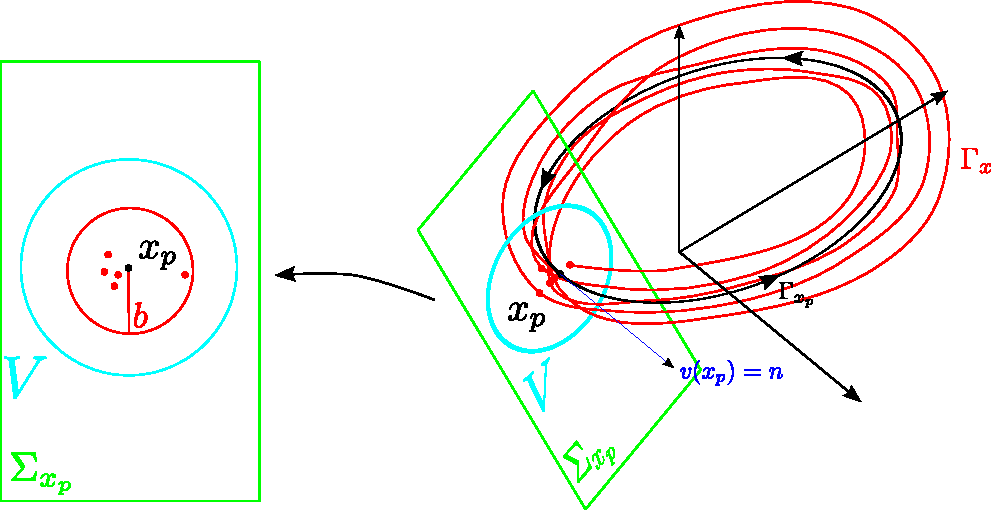
\includegraphics[width=1\textwidth]{img/periodische_orbits/stabilitaetskriterium.pdf}
		\caption{Illustration des Satzes "uber das Stabilit"atskriterium. $\Gamma_{x_p}$ ist orbital asymptotisch stabil. Kontinuierliche System (rechts); Das dazugeh"orige diskretisierte Poincar\'{e} System (links)}
\end{figure}

\begin{beispiel}
Betrachte folgende Differentialgleichung
\begin{align*}
	\begin{cases}
		&\dot x = \mu x - y - x(x^2+y^2)\\
		&\dot y = x + \mu y - y(x^2+y^2)
	\end{cases}
\end{align*}
mit einem Parameter $\mu > 0$. Eine Transformation in Polarkoordinaten vermittels $x = r \cos(\theta),\ y = r \sin(\theta), \ r\geq 0, \ \theta \in [0,2\pi)$ liefert
\begin{align*}
	\begin{cases}
		&\dot t = \mu r - r ^3\\
		& \dot \theta = 1
	\end{cases}
\end{align*}
Daher ist die Flussabbildung folgenderma"sen gegeben
$$\phi\left(t, \begin{pmatrix} r_0\\ \theta_0 \end{pmatrix}\right) = \begin{pmatrix}
	\left(\frac 1\mu + e^{-2\mu t}\left(\frac{1}{r_0^2} - \frac 1\mu\right)\right)^{-\frac 12}\\
	t + \theta_0
\end{pmatrix}$$
Ein periodischer Orbit $\Gamma$ ist offensichtlich gegeben durch 
\begin{align*}
\begin{cases}
 &r = \sqrt\mu\\
 &\theta = \theta_0
\end{cases}
\Leftrightarrow
\begin{cases}
 & x(t) = \sqrt\mu \cos\left(\theta(t)\right)\\
 & y(t) = \sqrt\mu \sin\left(\theta(t)\right)
\end{cases}
\end{align*}
Also hat dieser Orbit die Periode $2\pi$ und er besitzt die Poincar\'{e} Abbildung
$$ P_\Sigma (r_0) = \left(\frac 1\mu + e^{-2\mu t}\left(\frac{1}{r_0^2} - \frac 1\mu\right)\right)^{-\frac 12}$$
wobei $\Sigma = \RR\times\{0\}$, falls $\theta_0 \neq \frac{(2k+1)\pi}{2}$, ansonsten $\Sigma = \{0\}\times\RR$. F"ur alle $\mu > 0$ gilt $P_\Sigma(\sqrt \mu) = \sqrt \mu$. Die Ableitung von $P_\Sigma$ nach $r$ ist 
$$\frac{\mathrm d}{\mathrm dr} P_\Sigma(\sqrt \mu) = e^{-4 \pi \mu} \stackrel{\mu > 0} < 1$$
Die direkte Methode von Lyapunov liefert, dass $(\sqrt \mu, \theta_0)^T$ asymptotisch stabil ist im Sinne von Lyapunov und somit liefert \eqref{stabilitatskriterium_periodische_orbits}, dass $(\sqrt \mu, \theta_0)^T$ orbital asymptotisch stabil ist.
\end{beispiel}

\begin{figure}[htpb]
		\centering
		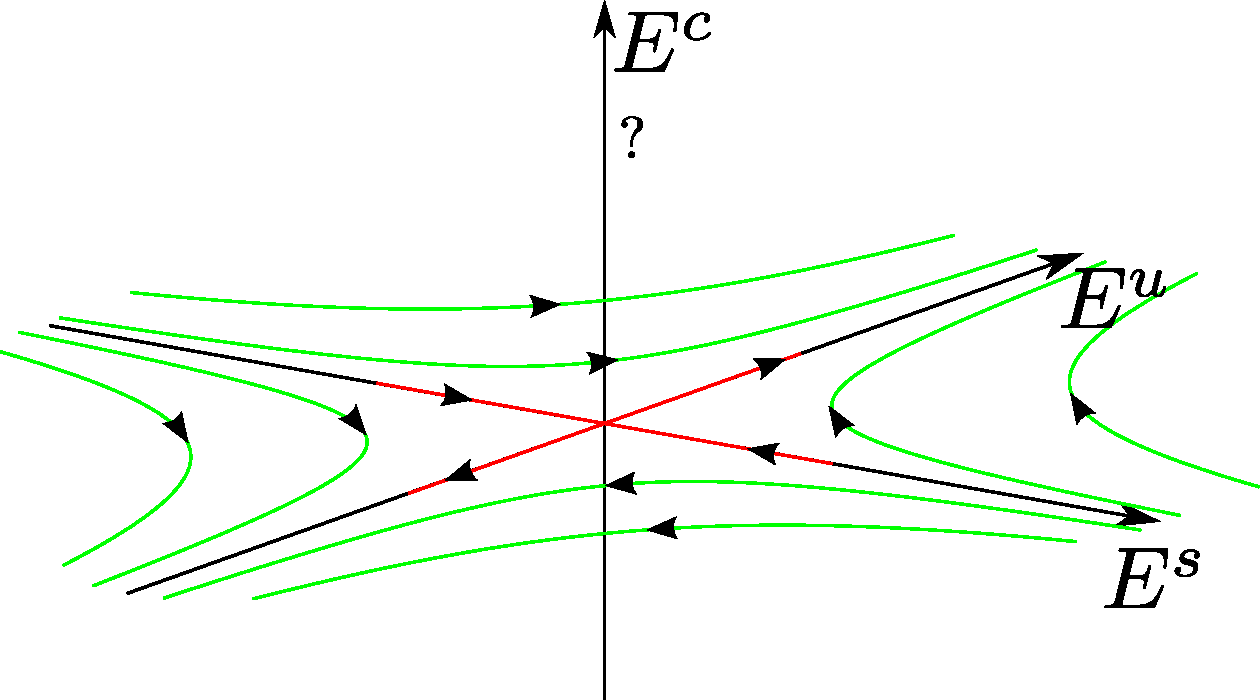
\includegraphics[width=0.5\textwidth]{img/periodische_orbits/beispiel_asymp_stabilitaet.pdf}
		\caption{Flussabbildung zum Beispiel}
\end{figure}


\section{Poincar\'{e}-Bendixson-Theorie}

Betrachte das GDG-System
	\[\dot{x} = v(x), \qquad x \in\mathbb{R} \]
\begin{definition}
	Sei \(\phi(t,x)\) Flu"sabbildung dieses Systems und \(x_0 \in \mathbb{R}\). Dann hei"st
		\[\omega(x_0)= \{x \in \mathbb{R}^n\ |\ \exists\  (t_j)_{j \in \mathbb{N}} \in \mathbb{R}, t_j \to \infty : \lim_{j\to \infty} \phi(t_j,x) = x_0\} \]
	\(\omega\)-Limesmenge des (Anfangs-) zustands \(x_0\). Jedes \(x \in \omega(x_0)\) ist ein 		sogenannter \emph{\(\omega\)-Limespunkt} von \(x_0\).

\end{definition}
\begin{description}
	\item[Bemerkung] Entsprechend definiert man \(\alpha\)-Limesmengen bzw. \(\alpha\)-Limespunkte im Fall \((t_j) \to -\infty\).
\end{description}

\begin{beispiel}
	\begin{enumerate}
		\item Sei \(x_G\) asymptotisch stabiler Gleichgewichtspunkt. Dann gilt \(\omega(x_0) = \{x_G\} \) f"ur alle \(x_0\) hinreichend nahe bei \(x_G\)
		\item Sei \(\Gamma_{x_p} \) ein orbital asymptotisch stabiler periodischer Orbit. Dann gilt \(\omega(x_0)= \Gamma_{x_p}\) f"ur alle \(x_0\) hinreichend nahe bei \(\Gamma_{x_p}\)
	\end{enumerate}
\end{beispiel}

\begin{definition}
Ein Orbit $\Gamma$ hei"st \emph{heterokliner Orbit} zwischen $x_1$ und $x_2$, falls ein \emph{heterokliner Punkt} $x_h \in \Gamma$ existiert, sodass 
\[\lim_{t\to -\infty} \phi(t,x_h) = x_1,\qquad \lim_{t\to\infty} \phi(t,x_h) = x_2\]
gilt. Seien \(x_G^1,...,x_G^N\) Gleichgewichtspunkte, $x_G^{N+1}$ bezeichne $x_G^1$. Seien $\Gamma_{k}$ heterokline Orbits zwischen $x_G^k$ und $x_G^{k+1}$ mit heteroklinen Punkt $x_h^k$. Dann hei"st die Menge 
	$$	\bigcup_{k=1}^{N} \Gamma_k \cup x_G^k$$
\emph{heterokliner Zykel}.
\end{definition}
\begin{description}
\item[Bemerkung] Es ist in der Definition eines heteroklinen Orbits auch zugelassen, dass dieser Orbit zwischen zwei gleichen Punkten verl"auft, d.h. $x_1 = x_2$. Ein solcher Orbit wird auch als \emph{homokliner Orbit} bezeichnet.
\end{description}
\begin{figure}[htpb]
		\centering
		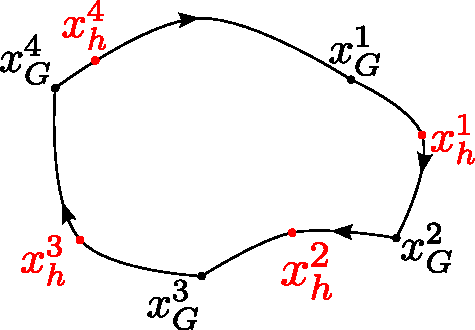
\includegraphics[width=0.4\textwidth]{img/poincare_Bendixson/heterokline_orbits.pdf}
		\caption{Illustration eines heteroklinen Zykels mit einem homoklinen Orbit zwischen $x_G^4$ und $x_G^5$}
\end{figure}


\begin{satz}[Poincar\'{e}-Bendixson-Theorem]
	Sei \(n=2, M \subset \mathbb{R}^2\) eine positiv invariante, kompakte Teilmenge. Dann gilt f"ur jedes \(x_0 \in M\) hinsichtlich der \(\omega\)-Limesmenge \(\omega(x_0)\) von \(x_0\) eine der folgenden drei Alternativen:
	\begin{enumerate}
		\item \(\omega (x_0) = \{x_G\} \) ist ein Gleichgewichtspunkt in M
		\item \(\omega(x_0) = \Gamma_{x_p}\) ist ein periodischer Orbit
		\item \(\omega(x_0)\) ist ein heterokliner Zykel
	\end{enumerate}

\end{satz}

\begin{corollar}
Es seien die Vorraussetzungen des Poincar\'{e}-Bendixson-Theorems gegeben. Ferner existiere in M kein Gleichgewichtspunkt des Systems. Dann enth"alt M mindestens einen periodischen Oribit des Systems.
\end{corollar}

\begin{beispiel}
	\begin{align*} \begin{cases}
		\dot{x} = \mu x - y - x(x^2+y^2) \\
		\dot{y} = x + \mu y - y(x^2+y^2)
	\end{cases} \end{align*}
	\(x=y=0\) ist trivialer (und einizger) Gleichgewichtspunkt. \\
	Betrachte das Vektorfeld \(v(x,y)\) des Systems l"angs eines Kreises \({x^2+y^2=R^2}\)
		\[\Rightarrow v(x,y) = \begin{pmatrix} \mu x - y - R^2x \\
		x + \mu y - R^2y \end{pmatrix} \]
		\begin{align*}
			\langle v(x,y), \begin{pmatrix} x \\ y \end{pmatrix} \rangle & = \mu x^2 - xy - R^2x^2 + xy + \mu y^2 - R^2y^2\\
			& = (\mu-R^2)(x^2+y^2) = (\mu - R^2)R^2 \lessgtr 0,\qquad ( R \gtrless \sqrt{\mu})
		\end{align*}
	Au"serhalb von \(x=y=0\) exisitiert kein weiterer Gleichgewichtspunkt, da \({\langle v(x,y),\begin{pmatrix} x \\ y \end{pmatrix} \rangle \not= 0}\) f"ur \(R\not= 0, \sqrt{\mu}\) und \(v_{|_{x^2+y^2=\mu}} = \begin{pmatrix} -y \\ x \end{pmatrix} \not= 0\).\\
	Somit existiert nach Poincar\'{e}-Bendixson innerhalb des Ringelements \newline \(R_1^2 < x^2+y^2 < R_2^2\) wenigstens \underline{ein} periodischer Orbit \(\Gamma_{x_p}\).
\end{beispiel}

\begin{figure}[htpb]
		\centering
		\includegraphics[width=0.4\textwidth]{img/poincare_Bendixson/beispiel_poincare_Bendixson.pdf}
		\caption{Vektorfeld auf den Kreisen $R_1$ sowie $R_2$ des obigen Beispiels}
\end{figure}
\section{Zeitlich periodische nicht-autonome GDG-Systeme}

Betrachte die Differentialgleichung
	\begin{align*} 
		&\dot{x} = v(t,x), \qquad x \in \mathbb{R}^n, t \in \mathbb{R}\ \text{mit} \\
		&v(t+T,x) = v(t,x)\qquad \forall (t,x) \in \mathbb{R}\times\mathbb{R}^n \\
	\end{align*}
wobei $T > 0$ minimal ist und die zeitliche Periode des System angibt. Da dies eine nicht-autonome Differentialgleichung ist, wird dadurch a priori kein dynamisches System erzeugt. Doch wenn man den erweiterten Phasenraum betrachtet wird ein dynamisches System induziert.
\begin{lemma}
Jede nicht-autonome Differentialgleichung $\dot x = v(t, x)$ kann folgenderma"sen in eine autonome Differentialgleichung 
transformiert werden
\begin{align*}
	\dot{\tilde x} := \dot{\begin{pmatrix}
		t\\
		x
	\end{pmatrix}} = 
	\begin{pmatrix}
		1\\
		v(t,x)
	\end{pmatrix} = 
	\begin{pmatrix}
		1\\
		v(\tilde x)
	\end{pmatrix}
	=: \tilde v(\tilde x)
\end{align*}
Dabei erweitert man den Phasenraum der nicht-autonomen Differentialgleichung auf $\RR \times \RR^n$, d.h. $\tilde v\colon \RR^{n+1} \to \RR^{n+1}$. Die L"osungen der autonomisierten Differentialgleichung mit Anfangswert $\tilde x (0) = \begin{pmatrix} \tau_0 \\ x_0 \end{pmatrix}$ entspricht der L"osung der nicht-autonomen Differentialgleichung mit Anfangswert $x(\tau_0) = x_0$.
\end{lemma}
Aus dem Lemma folgt sofort, dass die autonomisierte Differentialgleichung auf $\RR\times \RR^n$ ein dynamisches System induziert, falls $v$ entsprechende Bedingungen besitzt. Die Flussabbildung schreiben wir dann folgenderma"sen
\begin{align*} 
		\tilde x = \tilde\phi\left(t, \left(\tau_0, x_0\right) \right)
\end{align*}

Da $v$ in der ersten Komponente $T$-periodisch sind die L"osung mit Anfangswert $(\tau_0, x_0)$ identisch zu den L"osungen mit Anfangswert $(\tau_0 + kT, x_0)$ f"ur jedes $k\in\mathbb{Z}$. Daher ergibt sich auf kanonische Art eine Poincar\'{e}-Abbildung
\[P_{\tau_0} : \mathbb{R}^n \to \mathbb{R}^n, \ x_0\mapsto \phi(T;\tau_0,x_0) \]
wobei $\phi$ der Fluss der nicht-autonomen Differentialgleichung ist. Ein dazugeh"origer Poincar\'{e} Schnitt ist beispielsweise
$$ \Sigma_{\tau_0} = \left \{ \left. (t,x)\in\RR\times\RR^n \right | \langle (t - \tau_0 ,x), (1,0)\rangle = 0 \right \} = \left \{ \left . (\tau_0, x) \right| x \in \RR^n \right \} $$
Im folgenden werden wir diese spezielle Poincar\'{e} Abbildung auch mit \emph{Periodenabbildung} bezeichnen.
\begin{figure}[htpb]
		\centering
		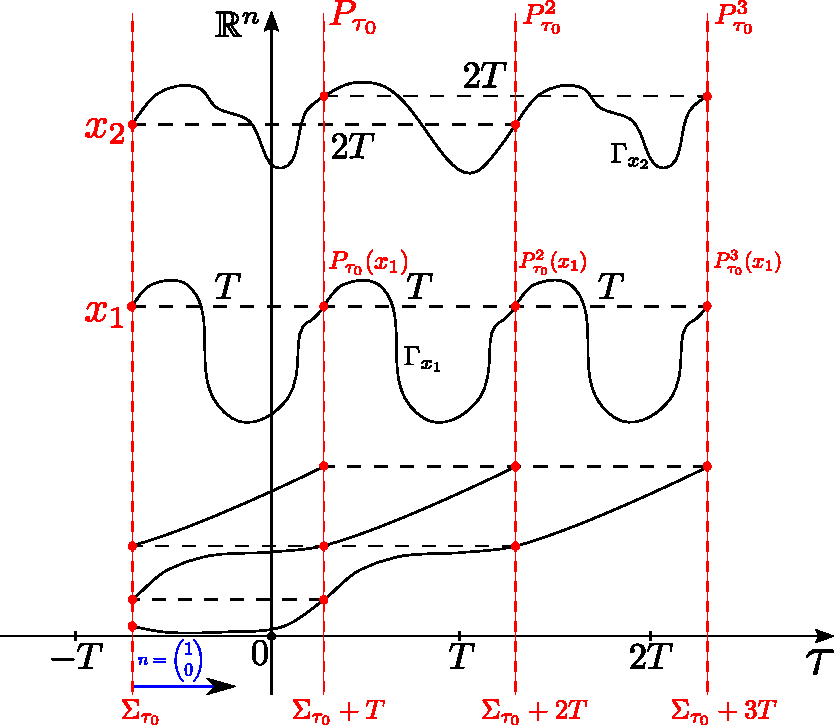
\includegraphics[width=0.7\textwidth]{img/poincare_Bendixson/periodenabbildung.pdf}
		\caption{Illustration der Periodenabbildung; $\Gamma_{x_1}$ ist $T$-periodisch, $\Gamma_{x_2}$ ist $2T$-periodisch}
\end{figure}


Die Periodenabbildung erzeugt analog wie im vorherigen Kapitel ein diskretes dynamisches System durch $\psi(k, x) = P_{\tau_0}^k(x)$. Daher kann man die periodischen Orbits von $\phi$ wieder mithilfe der Stabilit"at von Gleichgewichtspunkten von $\psi$ analysieren.

\begin{description}
	\item[Bemerkung] Fixpunkte von \(P_{\tau_0}\) entsprechen i.A. einem T-periodischen Orbit von \(\dot{x} = v(t,x) \) und Fixpunkte von \(P_{\tau_0}^K\) (\(K\in\mathbb{N}\)) entsprechen einem KT-periodischen Orbit einschlie"slich der Stabilt"atseigenschaften.
\end{description}

\begin{beispiel}
	\[\dot{x} = -x + \sin t \qquad (\text{nicht autom,} 2\pi \text{-periodisch})\]
	Die allgemeine homogene L"osung ist gegeben durch \(x_h(t) = e^{(t-t_0)}x_0\)
	Allgemeine L"osung: 
		\begin{align*} x(t) &= x_p(t) + x_h(t) \\
			& = \frac 1 2 (\sin t - \cos t) - \frac 1 2 e^{(t-t_0)}(\sin t_0 - \cos t_0) + e^{(t-t_0)}x_0\\
			&= \phi(t; t_0,x_0)
		\end{align*}
	\(\Rightarrow\) Mit \(\tau_0=t_0=0, t = 2\pi\) folgt:
		\begin{align*} P_0 : \mathbb{R} \to \mathbb{R}, x_0 \mapsto &-\frac 1 2 - \frac 1 2 e^{-2\pi}(-1)+e^{-2\pi}x_0\\
			& = -\frac 1 2 + \frac 1 2 e^{-2\pi} + e^{-2\pi}x_0
		\end{align*}
	ist Periodenabbildung f"ur obige GDG.\\
	Bestimmung des (eindeutigen) Fixpunkts: 
		\begin{align*} P_0(x_0)=x_0 &\Leftrightarrow -\frac 1 2 + \frac 1 2 e^{-2\pi} + e^{-2\pi}x_0 = x_0 \\
		&\Rightarrow x_0 = \frac{-\frac 1 2 + \frac 1 2 e^{-2\pi}} {e^{-2\pi}}
		\end{align*}
		\(\Rightarrow 0 < \frac{d}{d_x0} P_0(x_0) = e^{-2\pi}< 1 \Rightarrow\) asymptotisch stabil \(\Rightarrow\) obige GDG besitzt einen orbital asymptotisch stabilen \(2\pi\)-periodischen Orbit.
	
\end{beispiel}

%-----------------------------------------------------------------------------------------------

\chapter{Verzweigungstheorie (Bifurkationstheorie)}

Zunächst werden \emph{stationäre Verzweigungen} betrachtet.

\section{Kontinuierlicher Fall}

\subsection{$n=1$}

Für $(\lambda,x)\in\RR\times\RR$ und den \emph{Verzweigungsparameter} $\lambda$ betrachte man
\[
\dot x = v(\lambda,x).
\]

Bei der \emph{stationären Verzweigungstheorie} studiert man die Struktur der Gleichgewichtspunkte im Phasenraum ($x$-Raum) in Abhängigkeit vom Parameter $\lambda\in\RR$.

O.B.d.A.\ sei $x=0$ für alle Werte von $\lambda$ ein trivialer Gleichgewichtspunkt. Die Menge dieser trivialen Gleichgewichtspunkte bildet den \emph{Grundlösungszweig}. Falls der Grundlösungszweig die Form $x=x_G(\lambda)$ mit $\lambda\in\RR$ hat, setze
\[
x=x_G(\lambda)+\xi\Rightarrow\dot x = \dot\xi = v(\lambda,x_G(\lambda)+\xi) = \tilde v(\lambda,\xi).
\]
Da $v(\lambda, x_G(\lambda)) = 0$, ist $\xi = 0$ Gleichgewichtspunkt für alle $\lambda$

\begin{definition}
Ein Punkt $(\lambda_C,0)$ auf dem Grundlösungszweig heißt \emph{stationärer Verzweigungspunkt} des Problems $\dot x = v(\lambda, x)$, falls er in $\RR\times\RR$ Häufungspunkt nicht-trivialer Gleichgewichtslösungen $(\lambda,x_G)$ mit ${x_G\neq 0}$ ist.
\end{definition}

\begin{lemma}
Notwendige Bedingung für einen solchen Verzweigungspunkt (VP):
\[
v_x(\lambda_C,0) = 0\text{, falls }v\text{ } C^1\text{-glatt in beiden Variablen}
\]
\end{lemma}

\begin{beweis}
Angenommen $v_x(\lambda_C,0)\neq 0$. Dann hat $v(\lambda,x) = 0$ nahe $(\lambda_C, 0)$ zu jedem $\lambda$ genau einen Gleichgewichtspunkt $x=x_G(\lambda)$. Daher lässt sich der Satz über implizite Funktionen für $v(\lambda_C,0)$, $v_x(\lambda_C,0)$ mit $x_G(\lambda)$ $C^1$-glatt, $x(\lambda_C)=0$ anwenden. Damit gilt notwendigerweise $x_G(\lambda)\equiv 0$, d.h.\ nahe $(\lambda_C,0)$ existiert keine nicht-trivialen Lösungspunkte.
\end{beweis}

\begin{satz}[Hinreichende Bedingung für einen VP]
Sei $v$ $C^2$-Funktion ($k\geq 2$), $v(\lambda,0)=0$,
\begin{enumerate}
\item\label{enum:1}
$v_x(\lambda_C,0) = 0$

\item\label{enum:2}
$v_{\lambda x}(\lambda_C,0)\neq 0$.
\end{enumerate}
Dann ist $(\lambda_C,0)$ ein VP. Genauer: es existiert in der Nähe von $(\lambda_C,0)$ ein nicht-trivialer Lösungszweig $\lambda = \lambda^*(x)$ mit $|x|$ hinreichend klein, welcher den Grundlösungszweig in $(\lambda_C,0)$ \emph{transversal} schneidet, d.h.\ $\lambda^*(0) = \lambda_C$, und nicht-tangential zur $\lambda$-Achse in $(\lambda_C,0)$.

Gilt zudem
\begin{enumerate}
\setcounter{enumi}{2}
\item\label{enum:3}
$v_{xx}(\lambda_C,0)\neq 0$.
\end{enumerate}
Dann ist die Verzweigung bei $(\lambda_C,0)$ transkritisch, d.h.\ es gibt Werte $\lambda < \lambda_C$ als auch $\lambda > \lambda_C$, zu denen nicht-triviale Gleichgewichtspunkte existieren.

Falls anstelle von \ref{enum:3}
\begin{enumerate}
\setcounter{enumi}{3}
\item\label{enum:4}
\[
v_{xx}(\lambda_C,0) = 0\\
v_{xxx}(\lambda_C,0)\neq 0
\]
\end{enumerate}
mit $k\geq3$ gilt, dann ist die Verzweigung \emph{super- } bzw.\ \emph{subkritisch} je nach Vorzeichen von $v_{xxx}(\lambda_C,0)$ (\emph{Heugabelbedingung}).
\end{satz}

\begin{beweis}
Man betrachte die \emph{Gleichgewichtsbedingung (stationär)}
\[
v(\lambda,x) = 0.
\]
Setze
\[
V(\lambda,x) =
\begin{cases}
\frac{v(\lambda,x)}{x} & x\neq 0\\
v_x(\lambda,0) & x = 0
\end{cases}
\]
mit $(\lambda,x)\in\RR\times\RR$ beliebig, woraus die $C^{k-1}$-Glattheit von $V$ folgt ($k-1\geq 1$).

Aus \ref{enum:1} folgt $V(\lambda_C,0) = 0$. Ferner gilt $V_\lambda(\lambda_C,0)\neq 0$, weshalb sich $V(\lambda,x) = 0$ lokal eindeutig nach  $\lambda = \lambda^*(x)$ auflösen lässt (Satz über implizite Fuktionen) mit $\lambda^*(0) = \lambda_C$, $\lambda^*$ $C^{k-1}$-glatt.

Insbesondere gilt: $v(\lambda^*(x),x) = 0$ für alle $x\neq 0$

\underline{Taylorentwicklung} von $v(\lambda,x)$ um $(\lambda_C,0)$:
\begin{align*}
v(\lambda,x)&=\underbrace{a(\lambda)}_{v_x(\lambda,0)}x + \underbrace{b(\lambda)}_{\frac{1}{2}v_{xx}(\lambda,0)}x^2 + \underbrace{c(\lambda)}_{\frac{1}{6}v_{xxx}(\lambda,0)}x^3 + \dots\text{, falls } v \text{ entsprechend glatt}\\
&= v_{\lambda x}(\lambda_C,0)(\lambda-\lambda_C)x + \frac{1}{2}v_{xx}(\lambda,0)x^2 + \frac{1}{6}v_{xxx}(\lambda,0)x^3 + \dots
\end{align*}
Daraus folgt:
\[
V(\lambda,x) =  v_{\lambda x}(\lambda_C,0)(\lambda - \lambda_C) + \frac{1}{2}v_{xx}(\lambda,0)x + \frac{1}{6}v_{xxx}(\lambda,0)x^2 + \dots
\]
Daher gilt:
\begin{align*}
V_\lambda(\lambda_C,0) &= v_{\lambda x}(\lambda_C,0)\neq 0\\
V_x(\lambda_C,0) &= \frac{1}{2}v_{xx}(\lambda,0)\\
V_{xx}(\lambda_C,0) &= \frac{1}{6}v_{xxx}(\lambda,0)
\end{align*}

\underline{Zusatzaussage:}

Aus \ref{enum:3} folgt:
\begin{align*}
V(\lambda^*(x),x) &= 0\text{, für } |x| \text{ hinreichend klein}\\
V_x(\lambda^*(x),x) + V_\lambda(\lambda^*(x),x)\cdot(\lambda^*)'(x) &= 0
\end{align*}
Speziell für $x=0$ ergibt sich:
\[
V_x(\lambda_C,0) + \underbrace{V_\lambda(\lambda_C,0)}_{\neq 0\text{ wegen \ref{enum:2}}}\cdot(\lambda^*)'(0) = 0
\]
Somit gilt:
\[
(\lambda^*)'(0) = -\frac{V_x(\lambda_C,0)}{V_\lambda(\lambda_C,0)} = -\frac{v_{xx}(\lambda_C,0)}{2v_{\lambda x}(\lambda_C,0)}\stackrel{\ref{enum:3}}{\neq}0
\]
und $(\lambda_C,0)$ ist daher transkritischer VP.

Falls \ref{enum:4} gilt, ist $(\lambda^*)'(0) = 0$:
\begin{align*}
V_{x\lambda}(\lambda^*(x),x)\cdot(\lambda^*)'(x) + V_{xx}(\lambda^*(x),x) + V_{\lambda\lambda}(\lambda^*(x),x)\cdot(\lambda^*)'(x)^2\\
 + V_{\lambda x}(\lambda^*(x),x)\cdot(\lambda^*)'(x) + V_\lambda(\lambda^*(x),x)(\lambda^*)''(x) = 0
\end{align*}
Speziell für $x =0$ ergibt sich:
\[
V_{x\lambda}(\lambda_C,0)\cdot\underbrace{(\lambda^*)'(0)}_{= 0} + V_{xx}(\lambda_C,0) + V_{\lambda x}(\lambda_C,0)\cdot\underbrace{(\lambda^*)'(0)}_{= 0} + V_\lambda(\lambda_C,0)\cdot(\lambda^*)''(0)=0
\]
Letztendlich folgt daraus:
\[
(\lambda^*)''(0) = -\frac{V_{xx}(\lambda_C,0)}{V_\lambda(\lambda_C,0)} = -\frac{v_{xxx}(\lambda_C,0)}{6v_{\lambda x}(\lambda_C,0)}\neq 0
\]
\end{beweis}

\begin{bemerkung}
Diskreter Fall ($n = 1$):

Sei $\psi:\RR\times\RR\rightarrow\RR$ mit $\psi(\lambda,\cdot):\RR\rightarrow\RR$ Homöomorphismus ($C^k$-Diffeomorphismus)

$\psi(\lambda,0) = 0$ für alle $\lambda\in\RR$, d.h. $x = 0$ ist für alle $\lambda\in\RR$ ein trivialer Fixpunkt.

Nicht-triviale Gleichgewichtspunkte: $\psi(\lambda,x)=x\Leftrightarrow\underbrace{\psi(\lambda,x)-x}_{= v(\lambda,x)} = 0$
Das zugehörige stationäre Problem ist formal identisch mit jenem des kontinuierlichen Falls weshalb der Satz entsprechend anwendbar ist.
\end{bemerkung}

\begin{beispiel}
$\dot x = \lambda x - x^2$, $v(\lambda,0) = 0$ für alle $\lambda$, $\underbrace{v_x(\lambda,0)}_{= (\left.\lambda - 2x)\right|_{x = 0}}\stackrel{!}{=}0$.

Wegen \ref{enum:1} ist $\lambda = \lambda_C = 0$ kritischer Punkt (sonst nirgends VP).
\begin{align*}
v_{x\lambda}(\lambda_C,0) &= 1\neq 0\text{, daher ist } (\lambda_C,0)\text{ VP,}\\
v_{xx}(\lambda,0) &= -2,\,v_{xx}(0,0) = -2\neq 0\text{, daher ist }(\lambda_C,0) = (0,0)\text{ transkritischer VP.}
\end{align*}
\end{beispiel}
\end{document}
